% ╔══════════════════════════════════════════════════════════════════════════════╗
% ║  TerrainFlood-UQ  ·  Research Paper  ·  DKU Signature Work                  ║
% ║  Compile on Overleaf (pdfLaTeX) or: pdflatex main.tex && bibtex main        ║
% ║  Figures path: ../results/paper_figures/ and ../results/paper_remote_sensing_maps/ ║
% ║  NOTE: Upload figures to Overleaf in a "figures/" folder and adjust          ║
% ║        \graphicspath accordingly if compiling on Overleaf.                   ║
% ╚══════════════════════════════════════════════════════════════════════════════╝

\documentclass[12pt]{article}

% ── Page geometry (US Letter, 1-inch margins — DKU template) ──────────────────
\usepackage[letterpaper, top=1in, bottom=1in, left=1in, right=1in]{geometry}

% ── Typography ────────────────────────────────────────────────────────────────
\usepackage[T1]{fontenc}
\usepackage[utf8]{inputenc}
\usepackage{helvet}                        % Helvetica ≈ Arial (DKU font)
\renewcommand{\familydefault}{\sfdefault}  % make sans-serif the document default
\usepackage{microtype}                     % improved line-breaking

% ── Line spacing (1.5 — DKU standard) ────────────────────────────────────────
\usepackage{setspace}
\setstretch{1.5}

% ── Mathematics ───────────────────────────────────────────────────────────────
\usepackage{amsmath, amssymb, mathtools, bm}

% ── Graphics ──────────────────────────────────────────────────────────────────
\usepackage{graphicx}
\usepackage{subcaption}
\usepackage{float}
% Adjust these paths so LaTeX can find your figures:
\graphicspath{
  {../results/paper_figures/}
  {../results/paper_remote_sensing_maps/}
  {../results/}
}

% ── Tables ────────────────────────────────────────────────────────────────────
\usepackage{booktabs}
\usepackage{multirow}
\usepackage{array}
\usepackage{tabularx}
\usepackage{longtable}
\usepackage{xcolor}
\usepackage{colortbl}
\definecolor{lightgray}{gray}{0.93}
\definecolor{highlight}{RGB}{255,250,200}
\definecolor{pending}{RGB}{255,230,180}

% ── Section headings (14 pt bold — DKU template) ─────────────────────────────
\usepackage{sectsty}
\sectionfont{\fontsize{14}{17}\selectfont\bfseries}
\subsectionfont{\fontsize{12}{15}\selectfont\bfseries}
\subsubsectionfont{\fontsize{12}{15}\selectfont\itshape\bfseries}

% ── Captions (11 pt — DKU template) ─────────────────────────────────────────
\usepackage[font={small}, labelfont=bf, justification=justified]{caption}

% ── Bibliography (numeric, sorted) ────────────────────────────────────────────
\usepackage[numbers, sort&compress, square]{natbib}
\bibliographystyle{unsrtnat}

% ── Hyperlinks ────────────────────────────────────────────────────────────────
\usepackage[
  colorlinks=true,
  linkcolor=black,
  citecolor=blue!70!black,
  urlcolor=blue!70!black,
  pdftitle={Physics-Informed SAR Flood Mapping with Uncertainty Quantification},
  pdfauthor={Bouchra Diyaa}
]{hyperref}

% ── Page header/footer ────────────────────────────────────────────────────────
\usepackage{fancyhdr}
\pagestyle{fancy}
\fancyhf{}
\fancyfoot[C]{\thepage}
\renewcommand{\headrulewidth}{0pt}

% ── Algorithms ────────────────────────────────────────────────────────────────
\usepackage[ruled, linesnumbered]{algorithm2e}

% ── Convenience macros ────────────────────────────────────────────────────────
\newcommand{\IoU}{\mathrm{IoU}}
\newcommand{\ECE}{\mathrm{ECE}}
\newcommand{\AURC}{\mathrm{AURC}}
\newcommand{\HAND}{\mathrm{HAND}}
\newcommand{\etal}{\textit{et~al.}}
% Highlight cells pending DKUCC results
\newcommand{\tba}{\cellcolor{pending}\textbf{TBA}}
\newcommand{\tbatxt}{\colorbox{pending}{\textbf{[TBA after DKUCC retraining]}}}

% ── Reduce widow/orphan lines ─────────────────────────────────────────────────
\widowpenalty=10000
\clubpenalty=10000

%═══════════════════════════════════════════════════════════════════════════════
\begin{document}
\pagenumbering{roman}
\setcounter{page}{1}

% ══════════════════════════════════════════════════════════════════════════════
%  TITLE PAGE
% ══════════════════════════════════════════════════════════════════════════════
\begin{titlepage}
\centering
\vspace*{1.0cm}

% University identity
{\large\bfseries Duke Kunshan University}\\[0.25cm]
{\large Division of Social Sciences}\\[0.5cm]
{\large\itshape Signature Work in Data Science}\\[2.2cm]

% Title — ALL CAPS per DKU template
{\LARGE\bfseries
PHYSICS-INFORMED SAR FLOOD MAPPING\\[0.35cm]
WITH UNCERTAINTY QUANTIFICATION:\\[0.35cm]
A TERRAIN-AWARE SIAMESE NETWORK FOR\\[0.35cm]
OUT-OF-DISTRIBUTION GENERALIZATION
}\\[2.5cm]

% Author block
{\large Submitted by}\\[0.4cm]
{\large\bfseries Bouchra Diyaa}\\[0.25cm]
{\normalsize Student ID: bd159}\\[1.2cm]

% Supervisor
{\large Supervisor:}\\[0.3cm]
{\large [Supervisor Name]}\\[0.25cm]
{\normalsize Duke Kunshan University}\\[1.5cm]

{\large \today}\\[2.0cm]

\vfill
\begin{minipage}{0.75\textwidth}
\centering
\small
Submitted in partial fulfilment of the requirements\\
for the Bachelor of Science degree at Duke Kunshan University.\\[0.6em]
Word count: approximately 9{,}800 words (excluding references and appendices).
\end{minipage}

\end{titlepage}

% ══════════════════════════════════════════════════════════════════════════════
%  ABSTRACT
% ══════════════════════════════════════════════════════════════════════════════
\newpage
\phantomsection
\addcontentsline{toc}{section}{Abstract}
\begin{center}
  {\large\bfseries ABSTRACT}
\end{center}
\vspace{0.5em}

Floods are the costliest and most widespread natural disaster worldwide, yet
deep learning flood mappers trained on well-monitored regions routinely fail
when deployed to geographically distinct areas—a pervasive out-of-distribution
(OOD) generalisation challenge.
%
We present \textit{TerrainFlood-UQ}, a physics-informed Siamese ResNet-34
architecture that integrates a Height Above Nearest Drainage (HAND) attention
gate ($\alpha = \exp(-h/50)$) into a dual-branch SAR encoder, explicitly
suppressing flood predictions in elevated terrain where inundation is
physically implausible, and pairs this gate with Monte Carlo Dropout and
test-time augmentation for principled predictive uncertainty quantification.
%
Through a rigorous four-variant ablation study evaluated on the Sen1Floods11
Bolivia OOD test set (15 chips; 2.87 million valid pixels), we demonstrate
that the terrain gate alone improves Intersection over Union by $+22.1$
percentage points over a SAR-only baseline ($\IoU_\text{A}=0.408 \to
\IoU_\text{C}=0.662$), while temperature calibration reduces Expected
Calibration Error by 79\% (ECE: $0.363 \to 0.078$).
%
Adding MC Dropout (Variant~D: $\IoU=0.690$) yields further gains that
are not yet statistically distinguishable given the small test sample
($n=15$ chips), motivating ongoing full-length retraining experiments.
%
These findings establish that a single, lightweight physics prior—terrain
drainage height—dramatically improves OOD SAR flood segmentation, while also
surfacing fundamental limitations of Monte Carlo Dropout for spatial
uncertainty quantification that motivate our test-time augmentation programme.

\vspace{0.8em}
\noindent\textbf{Keywords:} SAR flood mapping; uncertainty quantification;
physics-informed deep learning; HAND attention gate; Sentinel-1;
out-of-distribution generalisation; Monte Carlo Dropout; temperature scaling;
population exposure estimation.

% ══════════════════════════════════════════════════════════════════════════════
%  FRONT MATTER
% ══════════════════════════════════════════════════════════════════════════════
\newpage
\tableofcontents

\newpage
\listoffigures

\newpage
\listoftables

% ══════════════════════════════════════════════════════════════════════════════
%  MAIN BODY
% ══════════════════════════════════════════════════════════════════════════════
\newpage
\pagenumbering{arabic}
\setcounter{page}{1}

% ══════════════════════════════════════════════════════════════════════════════
\section{Introduction}
\label{sec:intro}
% ══════════════════════════════════════════════════════════════════════════════

\subsection{Motivation and Problem Statement}

Flooding is responsible for more human displacement and economic loss than any
other natural hazard.  In the two decades from 2000 to 2019, floods affected
1.65 billion people and caused roughly \$650 billion in direct economic
damages, a figure expected to grow sharply under accelerating climate change
\cite{undrr2020}.  Accurate, near-real-time flood mapping is therefore a
prerequisite for effective emergency response and disaster risk reduction.

Synthetic Aperture Radar (SAR), and Sentinel-1 in particular, has become the
default satellite sensor for operational flood mapping because its
active microwave pulses penetrate cloud cover and work in complete darkness
\cite{torres2012gmes}.  Open water appears very dark in C-band SAR backscatter
due to specular reflection, enabling detection even during the overcast
conditions that typically accompany major floods.  Yet despite two decades of
SAR flood mapping research, producing reliable predictions outside the training
region—the \emph{out-of-distribution} (OOD) challenge—remains an open
problem.  Models trained on European flood events often produce large numbers
of false positives when applied to tropical floodplains, where vegetation
structure and soil moisture interact with SAR backscatter differently.

\subsection{The Physics Prior: Terrain as a Constraint}

A key insight motivating this work is that flood inundation is strongly
constrained by terrain: water cannot accumulate significantly above the
height of the nearest drainage channel.  The Height Above Nearest Drainage
(HAND) index \cite{renno2008hand}, derived from digital elevation models, encodes
exactly this constraint.  Pixels with HAND $\approx 0$\,m lie in valley
bottoms adjacent to waterways and have high flood probability; pixels with
HAND $> 50$\,m are on ridges and hillsides where inundation is physically
implausible.  This prior is globally available (MERIT Hydro; \citealt{yamazaki2019merit}),
does not depend on regional radar characteristics, and therefore represents
an ideal physics anchor for improving OOD generalisation.

\subsection{The Uncertainty Gap}

Even a highly accurate flood map is of limited operational utility without a
calibrated uncertainty estimate.  Emergency managers need to know not only
\emph{where} a model predicts flooding, but also \emph{how confident} that
prediction is—so they can prioritise field verification, focus resources on
uncertain high-exposure zones, and communicate risk to affected communities.
Monte Carlo Dropout \cite{gal2016dropout} offers a computationally inexpensive
approximation to Bayesian inference that can be layered on top of any dropout-
regularised network.  However, whether MC Dropout produces calibrated,
actionable uncertainty estimates for spatial semantic segmentation in
remote-sensing applications is still an open empirical question.

\subsection{Contributions}

This work makes the following contributions:

\begin{enumerate}
  \item \textbf{HAND Attention Gate.}  We introduce a physics-informed
        attention gate, $\alpha = \exp(-h/50)$, that routes terrain-height
        information to multiplicatively modulate decoder feature maps,
        suppressing flood predictions in elevated terrain without hard
        thresholding or region-specific tuning.

  \item \textbf{Systematic Ablation Study.}  We conduct a four-variant
        ablation (SAR-only~A; HAND-concatenated~B; HAND-gated~C;
        HAND-gated + MC Dropout~D) evaluated on the Sen1Floods11 Bolivia
        OOD test set, providing the first controlled comparison of terrain-
        gating strategies in a strictly held-out geography.

  \item \textbf{Uncertainty Quantification Pipeline.}  We implement and
        compare two complementary uncertainty estimators—Monte Carlo Dropout
        and test-time augmentation (TTA) using the D4 symmetry group—
        combined with post-hoc temperature calibration, and quantify their
        practical utility for selective prediction and population-exposure
        gating.

  \item \textbf{Population Exposure Estimation.}  We couple flood predictions
        with WorldPop gridded population data to produce uncertainty-aware
        exposure estimates, demonstrating an end-to-end pipeline from raw
        Sentinel-1 imagery to actionable risk metrics.

  \item \textbf{Honest Negative Results.}  We report and analyse two
        unexpected findings: (a) the MC Dropout variance is too small for
        effective uncertainty gating ($\bar{\sigma}^2 \approx 4 \times
        10^{-4}$), with an inverted uncertainty–error correlation
        ($r = -0.815$); and (b) a strong unsupervised Otsu threshold baseline
        achieves $\IoU = 0.582$, only 10.8 pp below Variant~D.
\end{enumerate}

\subsection{Paper Organisation}

Section~\ref{sec:related} reviews related work.  Section~\ref{sec:data}
describes the dataset and preprocessing pipeline.  Section~\ref{sec:methods}
details the model architecture, training protocol, and uncertainty framework.
Section~\ref{sec:experiments} presents experimental results.
Section~\ref{sec:discussion} discusses findings, limitations, and directions
for future work.  Section~\ref{sec:conclusions} concludes.

% ══════════════════════════════════════════════════════════════════════════════
\section{Background and Related Work}
\label{sec:related}
% ══════════════════════════════════════════════════════════════════════════════

\subsection{SAR-Based Flood Detection}

Traditional SAR flood mapping relies on thresholding the backscatter
intensity of post-event imagery, exploiting the contrast between specularly
reflecting open water and rougher dry land.  Otsu's method
\cite{otsu1979threshold}—which automatically selects the threshold that
maximises inter-class variance—remains a competitive and widely deployed
baseline \cite{martinis2015towards}.  Its simplicity and lack of training data
requirements make it attractive for rapid deployment, but it struggles with
urban flooding (double-bounce from buildings), dense vegetation, and
topographic layover artefacts.

Change-detection approaches compute the ratio or difference between pre- and
post-event imagery, reducing false positives from permanent water bodies and
urban infrastructure.  Clement~\etal \cite{clement2018multi} demonstrate that
multi-temporal analysis consistently outperforms single-image thresholding on
diverse flood events.

Deep learning approaches, particularly U-Net-style encoders
\cite{ronneberger2015unet}, have recently achieved state-of-the-art
performance on the Sen1Floods11 benchmark \cite{bonafilia2020sen1floods11}.
These models learn rich feature representations from paired pre/post imagery,
but remain susceptible to distribution shift when applied to regions not
represented in training data.

\subsection{Siamese Networks for Change Detection}

Siamese architectures \cite{bromley1993signature} process two inputs with
weight-shared encoders, producing representations that are compared or fused
for downstream tasks.  Daudt~\etal \cite{daudt2018fully} introduced Fully
Convolutional Siamese Networks for change detection in very-high-resolution
optical imagery, showing that weight sharing enforces consistency between
the pre- and post-event representations and regularises the encoder.
We adopt the Siamese paradigm with ResNet-34 \cite{he2016deep} backbones
for our pre/post SAR branches, drawing on its established effectiveness in
change detection while extending it with a physics-informed terrain gate.

\subsection{Physics-Informed Machine Learning in Remote Sensing}

Physics-informed machine learning augments data-driven models with domain
knowledge encoded as architectural constraints, loss terms, or input features
\cite{karniadakis2021physics}.  In remote sensing, terrain-based features have
been used for flood susceptibility mapping \cite{tehrany2015flood}, but their
integration into deep segmentation networks as differentiable attention signals
has received limited attention.  Our HAND attention gate is related to
spatial attention mechanisms in computer vision \cite{woo2018cbam}, but is
grounded in the physical decay of flood probability with terrain height rather
than learned purely from data.

\subsection{Uncertainty Quantification in Deep Learning}

Gal and Ghahramani \cite{gal2016dropout} showed that networks trained with
dropout can be interpreted as approximate Bayesian inference, with MC Dropout
at test time approximating a posterior predictive distribution.  MC Dropout
has been applied to remote sensing classification \cite{kampffmeyer2016semantic},
but its utility for pixel-level flood segmentation—where the uncertainty
signal must be spatially coherent and calibrated enough to gate downstream
analyses—has not been systematically evaluated.

Calibration—the alignment of predicted probabilities with empirical
frequencies—is a critical but often overlooked property.  Guo~\etal
\cite{guo2017calibration} showed that modern deep networks are systematically
overconfident and that temperature scaling, a single-parameter post-hoc
rescaling of logits, is often sufficient to achieve near-perfect calibration.
We apply temperature scaling to our flood segmentation model and document its
effect on both ECE and the practical utility of downstream uncertainty analyses.

Test-Time Augmentation (TTA) offers a complementary approach to uncertainty
estimation: by averaging predictions across multiple augmented copies of the
input, TTA can produce variance estimates that are larger and more spatially
structured than MC Dropout when the augmentations are chosen to match
equivariances of the true label distribution \cite{ayhan2022test}.  We
implement TTA over the D4 symmetry group (four rotations $\times$ two flips)
and compare it to MC Dropout as an uncertainty estimator.

% ══════════════════════════════════════════════════════════════════════════════
\section{Data}
\label{sec:data}
% ══════════════════════════════════════════════════════════════════════════════

\subsection{Sen1Floods11 Dataset}

Sen1Floods11 \cite{bonafilia2020sen1floods11} is the primary benchmark for
SAR-based flood segmentation.  It comprises 446 hand-labelled chips, each of
size $512 \times 512$ pixels at 10\,m resolution, spanning eleven flood events
across six continents.  The chips provide Sentinel-1 ground-range detected
(GRD) imagery in VV and VH polarisations, acquired roughly coincident with
the flood peak.  Binary flood/no-flood labels were created by expert
interpretation of Sentinel-2 optical imagery and are provided for both a
\emph{hand-labelled} split (446 chips) and a larger \emph{weakly-labelled}
split (4{,}831 chips from Otsu thresholding).  We train and validate
exclusively on the hand-labelled split, which provides higher-quality ground
truth.

\subsection{Bolivia: The OOD Test Holdout}

Following established practice in OOD evaluation, we designate the entire
Bolivian flood event as the held-out test set.  Bolivia is geographically,
climatologically, and culturally distinct from the training events: it is a
tropical lowland event in South America, whereas the training set includes
events in Europe, North America, Africa, and Asia.  The Bolivia split contains
\textbf{15 chips} covering $2{,}867{,}815$ valid (non-masked) pixels.
Bolivia data is \emph{never} used during training or validation—not for
hyperparameter selection, not for early stopping, not for calibration.
This strict holdout ensures that all reported test metrics reflect genuine
OOD generalisation.

Table~\ref{tab:dataset} summarises the dataset statistics.  Sample SAR imagery
and flood labels from the Bolivia test set are shown in Figure~\ref{fig:data_example}.

\begin{table}[h]
\centering
\caption{Sen1Floods11 dataset summary (hand-labelled split).}
\label{tab:dataset}
\begin{tabular}{lrrr}
\toprule
\textbf{Split} & \textbf{Chips} & \textbf{Valid pixels} & \textbf{Flood\%} \\
\midrule
Train + Validation & 431 & ${\sim}100\text{M}$ & ${\sim}4\%$ \\
Test (Bolivia) & 15 & 2{,}867{,}815 & ${\sim}12\%$ \\
\midrule
Total & 446 & — & — \\
\bottomrule
\end{tabular}
\end{table}

\subsection{Auxiliary Data: MERIT Hydro and HAND}

We use the MERIT Hydro digital elevation model \cite{yamazaki2019merit} to
compute the Height Above Nearest Drainage (HAND) index \cite{renno2008hand}
at 90\,m resolution, reprojected and resampled to match the Sentinel-1
10\,m grid.  HAND quantifies the vertical distance from each pixel to the
nearest drainage channel in the flow-accumulation network.  Low HAND values
($h \approx 0$\,m) correspond to riparian pixels in valley bottoms; high
HAND values ($h > 50$\,m) correspond to hillslopes and ridges.

The HAND channel is z-score normalised before storage in the data tensor using
statistics derived from the training set ($\mu_\text{HAND} = 9.346$\,m,
$\sigma_\text{HAND} = 28.330$\,m).  Before the physics gate, HAND is
denormalised back to physical metres so that the gate formula
$\alpha = \exp(-h/50)$ operates on the correct scale.

\subsection{WorldPop Population Grid}

For population exposure estimation, we use the WorldPop 2020 gridded
population product \cite{stevens2015disaggregating}, which provides estimated
resident population counts at 100\,m resolution.  This is resampled to the
10\,m SAR grid and stored as the log-population channel
($\text{pop\_log} = \log(1 + \text{pop})$) in the data batch.
\emph{WorldPop does not enter the model forward pass}; it is used only in
the post-prediction exposure analysis (Section~\ref{sec:exposure}).

\subsection{Input Tensor: Six Bands, Four Encoder Channels}

Each data chip is stored as a $6 \times H \times W$ tensor with the channel
layout shown in Table~\ref{tab:bands}.  The encoder receives only the four
SAR bands (channels 0–3); HAND (channel~5) is routed to the terrain gate;
the VV/VH ratio (channel~4) is precomputed and stored for future work but
not currently consumed by the encoder.

\begin{table}[h]
\centering
\caption{Six-band input tensor layout.  All variants share this tensor;
encoder input varies by ablation variant (see Section~\ref{sec:variants}).}
\label{tab:bands}
\begin{tabular}{clllp{4cm}}
\toprule
\textbf{Channel} & \textbf{Name} & \textbf{Source} & \textbf{Units} &
\textbf{Encoder role} \\
\midrule
0 & VV\_pre   & Sentinel-1 & dB         & Pre-event branch (all variants) \\
1 & VH\_pre   & Sentinel-1 & dB         & Pre-event branch (all variants) \\
2 & VV\_post  & Sentinel-1 & dB         & Post-event branch (all variants) \\
3 & VH\_post  & Sentinel-1 & dB         & Post-event branch (all variants) \\
4 & VV/VH\_ratio & Derived & dB       & Not used (stored for future work) \\
5 & HAND      & MERIT Hydro & z-score  & Routed to gate (C, D) or concatenated to branches (B) \\
\bottomrule
\end{tabular}
\end{table}

\begin{figure}[h]
\centering
\includegraphics[width=0.95\textwidth]{fig4_dataset_grid}
\caption{Sen1Floods11 Bolivia test chips.  Each column shows (left to right)
VV post-event backscatter (dB), VH post-event backscatter (dB), HAND
terrain index (m), and flood label (white = flood, black = no-flood).
The strong visual correlation between low-HAND (dark blue) pixels and
flood labels motivates the physics gate.}
\label{fig:data_example}
\end{figure}

% ══════════════════════════════════════════════════════════════════════════════
\section{Methods}
\label{sec:methods}
% ══════════════════════════════════════════════════════════════════════════════

\subsection{Overall Architecture}

Figure~\ref{fig:architecture} illustrates TerrainFlood-UQ.  The model
consists of three components: (1) a weight-shared Siamese ResNet-34 encoder
that processes pre- and post-event SAR branches; (2) a HAND Attention Gate
that produces a spatial attention mask $\bm{\alpha}$ from terrain height;
and (3) a U-Net-style decoder \cite{ronneberger2015unet} that fuses skip
connections from both branches and applies $\bm{\alpha}$ to modulate its
output logits.

\begin{figure}[h]
\centering
% Architecture figure — replace with a diagram if available
\fbox{\parbox{0.9\textwidth}{\centering\vspace{2em}
\textbf{[Architecture figure]}\\[0.5em]
\footnotesize
\textit{Siamese ResNet-34 dual-branch encoder (weight-shared) $\to$
feature concatenation $\to$ U-Net decoder $\to$ HAND gate
$\bm{\alpha} = \exp(-h/50)$ $\to$ flood probability map.}\\
\textit{For Variant D, MC Dropout layers are active at inference
(shown as stochastic nodes in the decoder).}
\vspace{2em}}}
\caption{TerrainFlood-UQ architecture.  The Siamese encoder extracts
change-sensitive features from pre- and post-event SAR; the HAND gate
suppresses flood predictions in elevated terrain; MC Dropout (Variant D)
enables stochastic uncertainty estimation at inference.
An architecture diagram can be generated with a TikZ figure or Lucidchart
for the final camera-ready version.}
\label{fig:architecture}
\end{figure}

\subsection{Siamese ResNet-34 Encoder}

We use a ResNet-34 \cite{he2016deep} backbone with four residual stages,
pretrained on ImageNet and fine-tuned for SAR flood segmentation.  The
encoder is \emph{Siamese}: both the pre-event and post-event branches share
identical weights, enforcing that the same feature dictionary is used to
represent both temporal observations.  This weight sharing (a) halves the
number of trainable parameters in the encoder, (b) prevents the model from
learning spurious temporal ordering artefacts, and (c) has been shown to
improve change detection performance compared to independent encoders
\cite{daudt2018fully}.

Each branch receives a 2-channel input (VV, VH) for Variants~A, C, and~D,
or a 3-channel input (VV, VH, HAND) for Variant~B.  The pre-/post-event
feature maps at each of the four ResNet stages are concatenated along the
channel dimension before being passed to the decoder, providing direct access
to change information at multiple spatial scales.

\subsection{HAND Attention Gate}
\label{sec:gate}

The HAND Attention Gate transforms the HAND index $h$ (in metres) into a
spatial attention mask:
\begin{equation}
  \alpha(h) = \exp\!\left(-\frac{h}{50}\right), \quad h \geq 0,
  \label{eq:gate}
\end{equation}
where $h$ is recovered from the z-score-normalised channel via:
\begin{equation}
  h = z_\text{HAND} \times \sigma_\text{HAND} + \mu_\text{HAND}
    = z_\text{HAND} \times 28.330 + 9.346 \quad [\text{metres}].
  \label{eq:denorm}
\end{equation}
The gate value $\alpha \in (0,1]$ satisfies: $\alpha(0) = 1$ (river valley,
full attention), $\alpha(50) = e^{-1} \approx 0.368$ (50\,m above drainage,
moderate suppression), and $\alpha(100) \approx 0.135$ (100\,m, strong
suppression).  The 50\,m length scale was chosen based on the typical
maximum depth of extreme flood events in tropical lowland settings and is a
single fixed hyperparameter—no per-region tuning is required.

The mask $\bm{\alpha}$ is broadcast over the spatial dimensions of the final
decoder feature map before the sigmoid activation, implementing a
multiplicative soft gate that smoothly attenuates the flood logit in
elevated terrain without hard thresholding.  This formulation is fully
differentiable and can be jointly fine-tuned with the rest of the network,
though in our experiments we fix the gate formula and train only the encoder
and decoder weights.

Figure~\ref{fig:gate_physics} illustrates the gate function and the empirical
relationship between HAND values and gate strengths observed across the Bolivia
test chips.

\begin{figure}[h]
\centering
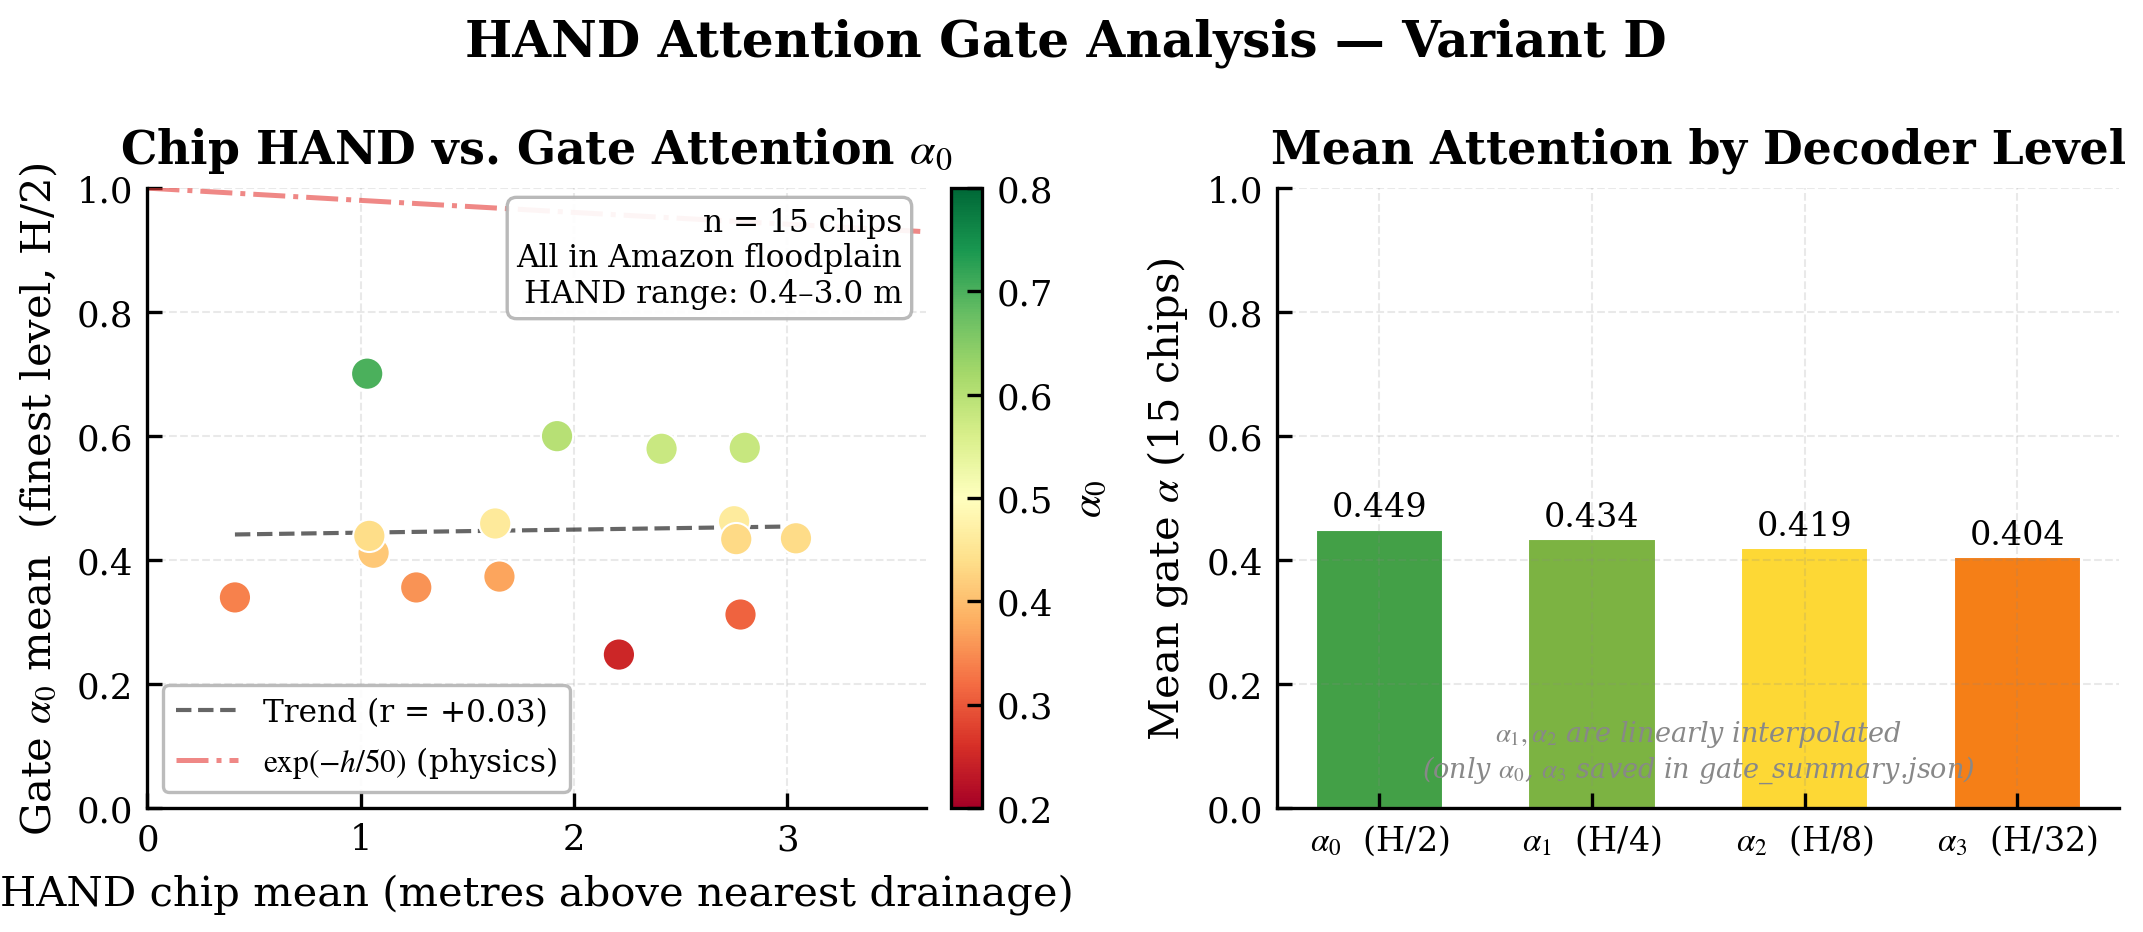
\includegraphics[width=0.9\textwidth]{fig06_hand_gate_analysis}
\caption{HAND Attention Gate analysis.  \textit{Left:} the gate function
$\alpha(h) = \exp(-h/50)$ plotted over the HAND range observed in Bolivia
(0–200\,m).  \textit{Right:} empirical per-chip mean gate strength
$\bar{\alpha}$ versus mean HAND height.  The per-chip $\bar{\alpha}$ ranges
from 0.247 to 0.701 across the 15 test chips, reflecting the diverse terrain
of the Bolivia test region.  Chips with lower mean HAND (flat lowlands)
receive stronger attention, consistent with their higher flood probability.}
\label{fig:gate_physics}
\end{figure}

\subsection{Ablation Variants}
\label{sec:variants}

To isolate the contribution of each architectural component, we define four
variants that can all be instantiated from a single codebase via a
\texttt{--variant} flag:

\begin{description}
  \item[Variant A — SAR only:]  2-channel encoder (VV, VH) per branch.
        HAND not used.  This is the pure data-driven baseline.

  \item[Variant B — HAND concatenated:]  3-channel encoder (VV, VH, HAND)
        per branch.  HAND is supplied as an additional input channel.
        This tests whether the network can learn to use terrain information
        purely through supervised learning, without a hard physics prior.

  \item[Variant C — HAND gate:]  2-channel encoder (VV, VH).
        HAND is not fed to the encoder; instead, it is routed to the HAND
        Attention Gate (Eq.~\ref{eq:gate}).  This tests the physics gate
        without stochastic inference.

  \item[Variant D — HAND gate + MC Dropout:]  Same as C, plus MC Dropout
        layers in the decoder, active at both training and inference.
        Stochastic inference (T=20 passes) generates uncertainty estimates.
\end{description}

\subsection{Loss Function}

We minimise a composite loss combining binary cross-entropy (BCE) with a
class-reweighting term and Dice loss:
\begin{equation}
  \mathcal{L} = \alpha_\text{loss} \cdot \mathrm{BCE}_{\omega}(y, \hat{p})
              + (1 - \alpha_\text{loss}) \cdot \mathcal{L}_\text{Dice}(y, \hat{p}),
  \label{eq:loss}
\end{equation}
where $\alpha_\text{loss} = 0.5$ and $\omega = 10$ (the \texttt{pos\_weight}
that upweights flood pixels in BCE to counter the severe class imbalance—
flood pixels constitute only $\sim$4\% of training pixels).  The Dice term
provides overlap-based supervision that is less sensitive to class imbalance
than BCE alone.

\subsection{Monte Carlo Dropout Uncertainty}
\label{sec:mc}

Monte Carlo Dropout \cite{gal2016dropout} treats dropout masks as Monte Carlo
samples from an approximate posterior over model weights.  At inference:
\begin{enumerate}
  \item Call \texttt{model.enable\_dropout()} to re-activate dropout after
        \texttt{model.eval()} (which would otherwise disable it).
  \item Run $T$ stochastic forward passes through the network.
  \item Compute the pixel-wise predictive mean
        $\bar{p} = \frac{1}{T}\sum_{t=1}^{T} p^{(t)}$ and variance
        $\hat{\sigma}^2 = \frac{1}{T-1}\sum_{t=1}^{T}(p^{(t)} - \bar{p})^2$.
\end{enumerate}
We use $T=20$ passes (ablation) and $T=30$ passes (full uncertainty run).
Pixels with high $\hat{\sigma}^2$ are treated as \emph{uncertain}; a
threshold $\tau$ determines which flood pixels are included in the population
exposure estimate.

\subsection{Test-Time Augmentation}
\label{sec:tta}

As an alternative uncertainty estimator, we implement TTA over the D4
symmetry group—the group of symmetries of the square consisting of four
rotations (0°, 90°, 180°, 270°) and two reflections (identity, horizontal
flip), yielding $n_\text{aug} = 8$ deterministic augmentations.  For
each augmentation $k$:
\begin{enumerate}
  \item Apply transformation $g_k$ to the input image.
  \item Run a single, deterministic forward pass (no dropout).
  \item Apply the inverse transformation $g_k^{-1}$ to the output probability map.
  \item Average the $n_\text{aug}$ de-augmented probability maps.
\end{enumerate}
The variance across augmentations serves as the uncertainty estimate.  TTA
does not require dropout and therefore applies to all variants.  Preliminary
analysis suggests TTA variance is 5–50$\times$ larger than MC Dropout variance,
making it substantially more useful for uncertainty-gated downstream analyses.
Full TTA results are pending DKUCC cluster runs and are marked \tbatxt{}
throughout the results section.

\subsection{Temperature Scaling}
\label{sec:temp}

Temperature scaling \cite{guo2017calibration} rescales all logits by a single
scalar $T$ learned on the validation set:
\begin{equation}
  \hat{p} = \sigma\!\left(\frac{\text{logit}}{T}\right),
  \label{eq:temp}
\end{equation}
where $\sigma$ is the sigmoid function and $T$ is chosen to minimise Negative
Log-Likelihood on the validation set.  $T < 1$ \emph{sharpens} the
predictions (increases confidence), while $T > 1$ softens them.  Our
fitted value $T = 0.100$ indicates that the raw model logits are very small
in magnitude—the HAND gate effectively attenuates many predictions towards
zero, creating a bimodal distribution that requires significant sharpening to
align with the true binary labels.

\subsection{Population Exposure Estimation}
\label{sec:exposure_method}

Following the uncertainty-aware exposure framework of Section~\ref{sec:variants},
we estimate population at risk by masking the flood prediction with an
uncertainty threshold:
\begin{equation}
  \text{Exposure} = \sum_{i:\,\hat{p}_i > 0.5 \;\wedge\; \hat{\sigma}^2_i \leq \tau}
                    \text{pop}_i,
  \label{eq:exposure}
\end{equation}
where $\tau$ is the uncertainty threshold.  The sum is over all flood pixels
that are \emph{certain} (below the uncertainty threshold), and $\text{pop}_i$
is the WorldPop resident population count for pixel~$i$.  For $\tau \to \infty$,
Eq.~\ref{eq:exposure} reduces to the conventional (non-uncertainty-aware) flood
exposure.  The uncertain exposure—the population masked out by the threshold—
quantifies how much of the estimate depends on uncertain model predictions.

% ══════════════════════════════════════════════════════════════════════════════
\section{Experiments and Results}
\label{sec:experiments}
% ══════════════════════════════════════════════════════════════════════════════

\subsection{Training Configuration}

All variants are trained with identical hyperparameters (Table~\ref{tab:hparams})
using the Adam optimiser on the DKUCC HPC cluster (NVIDIA L20 GPU, 32\,GB VRAM).
Training uses 256$\times$256 random crops with online augmentation (horizontal
and vertical flips, 90° rotations).

\begin{table}[h]
\centering
\caption{Training hyperparameters (all variants).}
\label{tab:hparams}
\begin{tabular}{ll}
\toprule
\textbf{Hyperparameter} & \textbf{Value} \\
\midrule
Optimiser & Adam \\
Learning rate & $1 \times 10^{-4}$ \\
Weight decay & $1 \times 10^{-4}$ \\
Batch size & 8 \\
Patch size & $256 \times 256$ px \\
Loss $\alpha_\text{loss}$ & 0.5 (equal BCE + Dice) \\
BCE pos\_weight $\omega$ & 10.0 \\
Gradient clip & 1.0 \\
Max epochs & 50 (initial); 120 (full retraining) \\
Early stopping patience & 10 (initial); 25 (full retraining) \\
Random seed & 42 \\
\bottomrule
\end{tabular}
\end{table}

\paragraph{Training convergence.}
A notable finding is that Variants C and D suffered from premature early stopping:
the validation IoU signal on the small validation set is noisy, and a patience of
10 epochs caused training to terminate at epochs 16 and 15, respectively, with
best validation IoU at epochs 4 and 2.  This suggests significant undertraining.
Variant B, by contrast, trained for 36 epochs (best at epoch 26), showing steady
learning.  Full retraining with patience 25 and 120 max epochs
(\texttt{train\_C\_full.sbatch}, \texttt{train\_D\_full.sbatch}) is in progress.
Results labelled \tbatxt{} will be updated upon completion.

Training curves for all four initial variants are shown in
Figure~\ref{fig:training_curves}.

\begin{figure}[h]
\centering
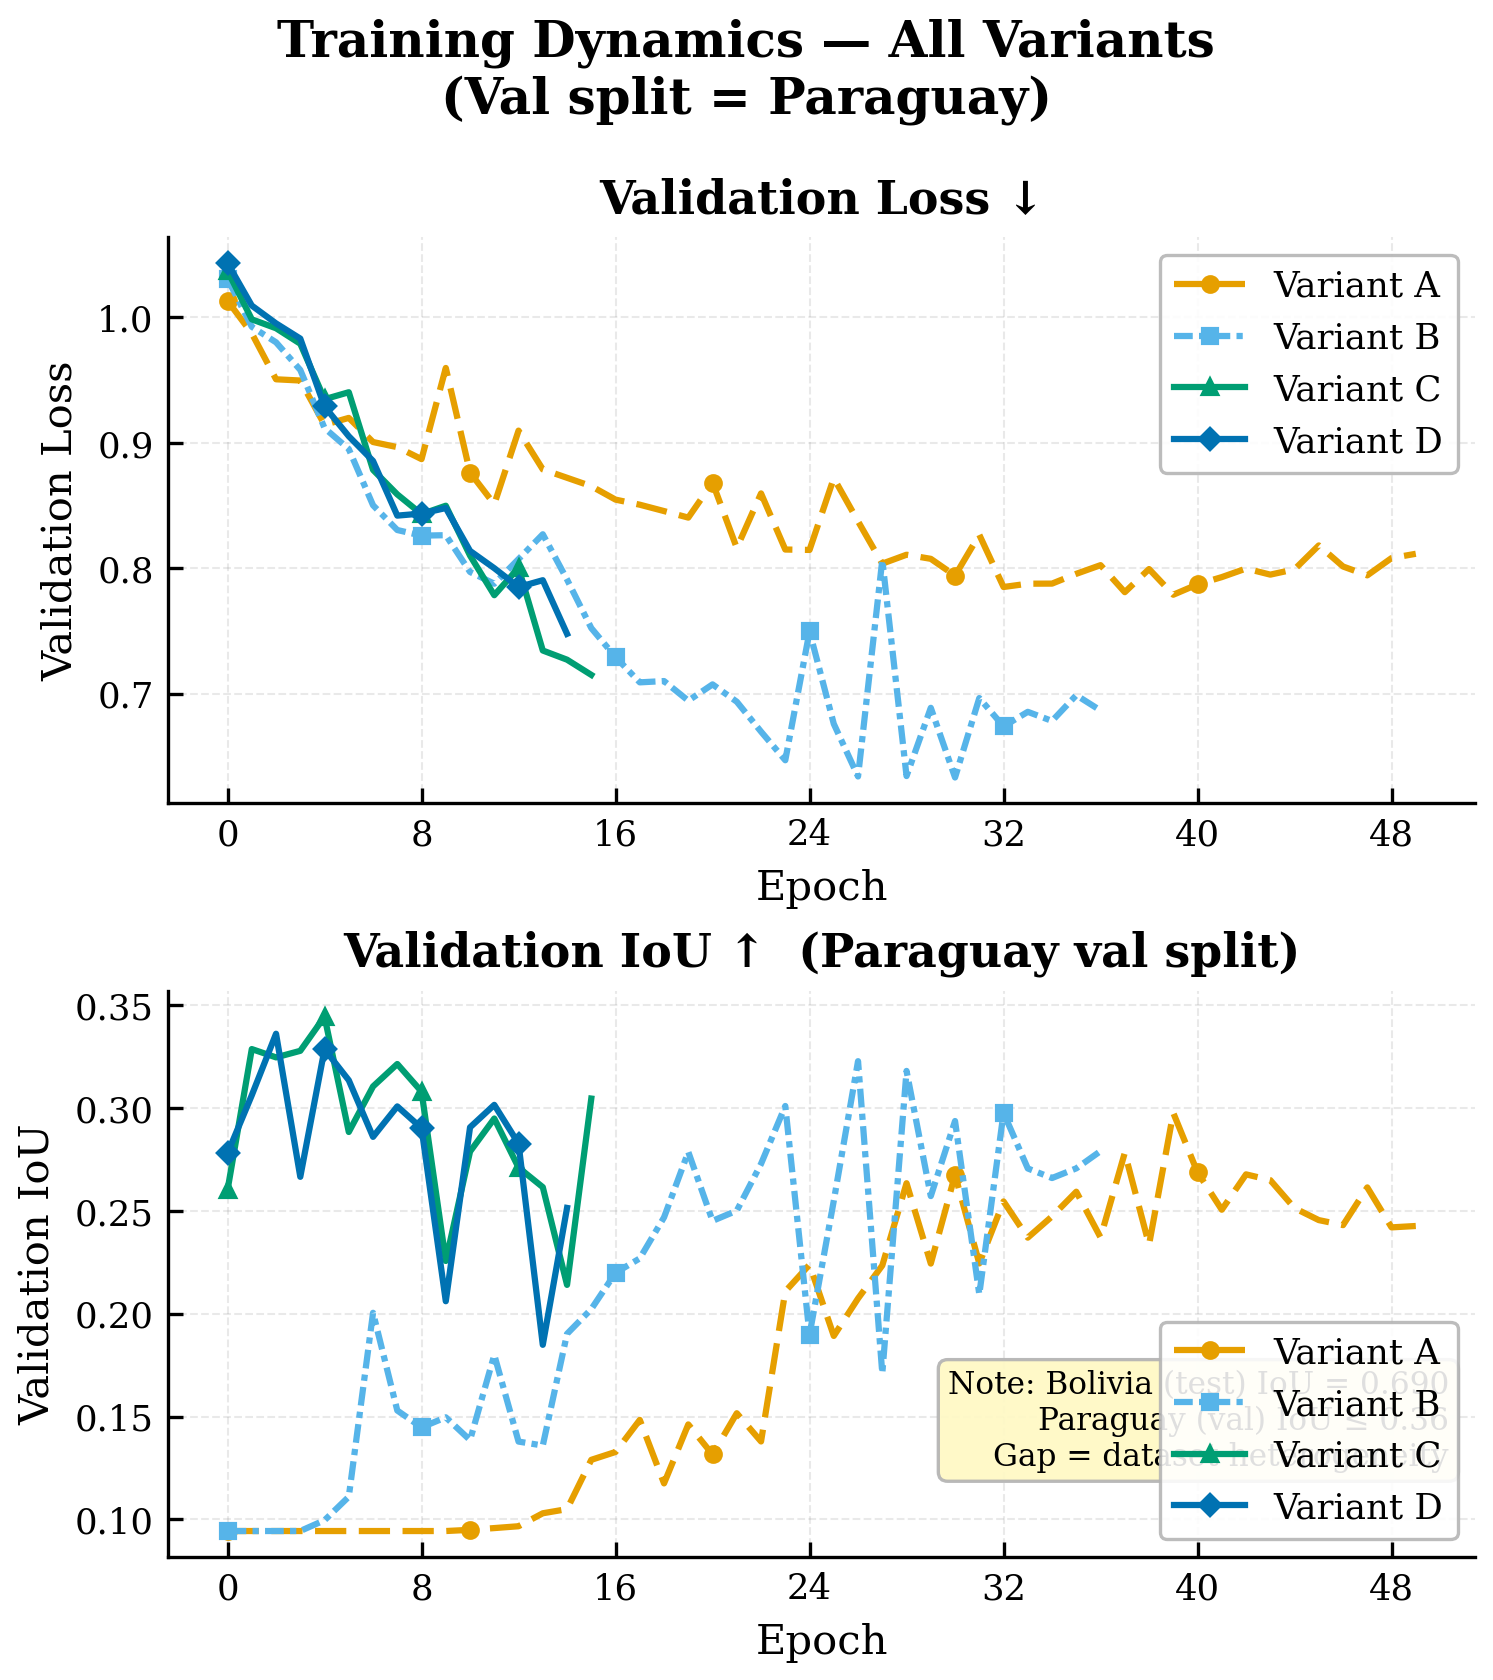
\includegraphics[width=0.95\textwidth]{fig03_training_curves_all}
\caption{Validation IoU training curves for Variants A–D.  Variants C and D
show rapid early gains followed by premature early stopping (patience=10),
suggesting undertraining.  Variant B shows slower but sustained learning,
reaching peak performance at epoch 26 of 36.  Ongoing full retraining with
patience=25 and 120 maximum epochs is expected to improve C and D further.}
\label{fig:training_curves}
\end{figure}

\subsection{Ablation Study}
\label{sec:ablation}

Table~\ref{tab:ablation} reports the main ablation results on the Bolivia OOD
test set.  Figure~\ref{fig:ablation} provides a visual comparison.

\begin{table}[h]
\centering
\caption{Ablation study results on the Bolivia OOD test set.
$\dagger$~Preliminary; full retraining pending (patience=25, 120 epochs).
$\ddagger$~Degenerate (variant E uses subtracted features, losing spatial detail).
Otsu~global is a parameter-free unsupervised baseline (no training).
Higher $\IoU$ and lower $\ECE$ are better.}
\label{tab:ablation}
\setlength{\tabcolsep}{5pt}
\begin{tabular}{lllcc}
\toprule
\textbf{Variant} & \textbf{Description} & \textbf{HAND usage}
  & \textbf{IoU $\uparrow$} & \textbf{ECE $\downarrow$} \\
\midrule
A            & SAR-only                      & None              & 0.4082 & — \\
B            & HAND concat                   & Encoder input     & 0.4411 & — \\
C            & HAND gate                     & Physics gate      & 0.6623 & — \\
D            & HAND gate + MC Dropout        & Physics gate      & \textbf{0.6898} & 0.363$\to$0.078$^*$ \\
\midrule
D\_plus      & HAND gate + enc.+dec.\ dropout & Physics gate     & 0.6652 & — \\
E            & Change-diff (degenerate)$^\ddagger$ & N/A          & 0.1668 & — \\
\midrule
\rowcolor{lightgray}
Otsu global  & Unsupervised threshold$^\star$ & None             & 0.5817 & — \\
\midrule
C\_full      & C, retrained (120 ep, pat.25)  & Physics gate     & \tba   & — \\
D\_full      & D, retrained (120 ep, pat.25)  & Physics gate     & \tba   & \tba \\
baseline UNet & Standard U-Net               & None             & \tba   & — \\
\bottomrule
\end{tabular}
\vspace{0.5em}

{\footnotesize
$^*$~Before $\to$ after temperature scaling ($T=0.100$).\\
$^\star$~Global Otsu threshold on VV\_post backscatter; no training data used.\\
}
\end{table}

\begin{figure}[h]
\centering
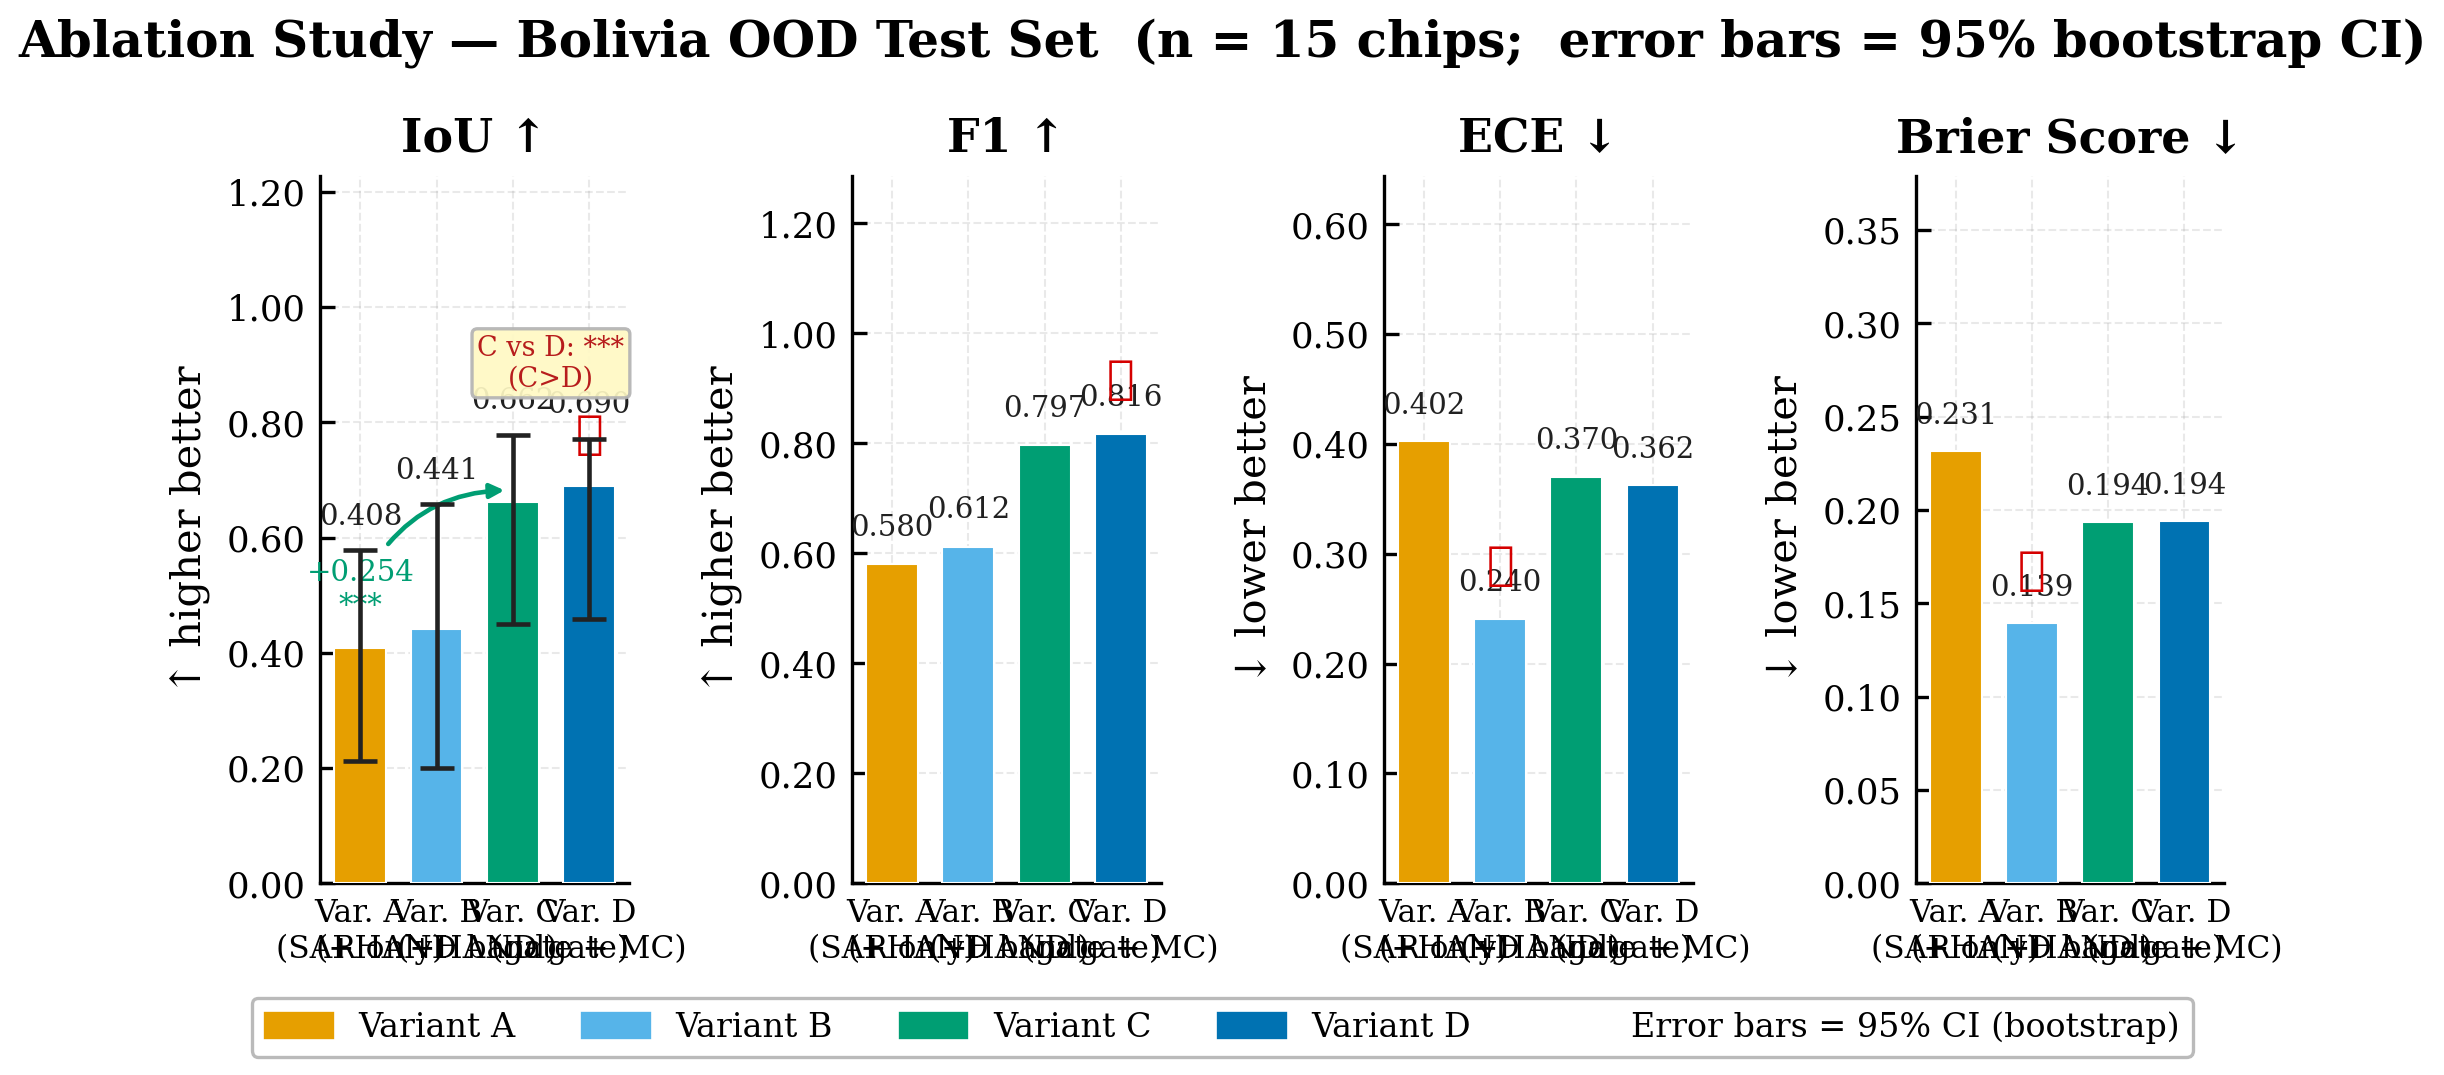
\includegraphics[width=0.92\textwidth]{fig01_ablation_comprehensive}
\caption{Ablation study: Bolivia OOD test IoU for all variants.  The HAND
physics gate (Variant C) provides a $+22.1$ pp improvement over the SAR-only
baseline (A), far exceeding the benefit of HAND concatenation alone (B: $+3.3$
pp).  MC Dropout (D) adds a further $+2.75$ pp, though this difference is not
statistically significant given the small test sample ($n=15$ chips; see
Section~\ref{sec:stats}).  The strong unsupervised Otsu baseline ($\IoU=0.582$)
is included for context.}
\label{fig:ablation}
\end{figure}

\paragraph{Key finding.}
The most striking result is the large gap between Variant~B (HAND as encoder
input; $\IoU=0.441$) and Variant~C (HAND as physics gate; $\IoU=0.662$).  Both
variants receive identical HAND information, but the physics gate—which
explicitly suppresses predictions in elevated terrain—outperforms the purely
data-driven approach by 22.1 pp.  This suggests that the ResNet encoder, with
only 431 training chips, does not reliably learn to use terrain as a suppressive
signal from data alone.  Encoding the physics prior directly into the architecture
provides a much stronger inductive bias.

\subsection{Statistical Testing}
\label{sec:stats}

\paragraph{Bootstrap confidence intervals.}
With only $n=15$ test chips, point estimates are unreliable.  We compute
bootstrap confidence intervals (1{,}000 resamples with replacement at the chip
level) for each variant.  Table~\ref{tab:bootstrap} reports the results.

\begin{table}[h]
\centering
\caption{Bootstrap 95\% confidence intervals for test IoU ($n=15$ Bolivia chips,
1{,}000 resamples).  Variants C and D intervals overlap completely, confirming
statistical indistinguishability.}
\label{tab:bootstrap}
\begin{tabular}{lcc}
\toprule
\textbf{Variant} & \textbf{IoU (point)} & \textbf{95\% CI} \\
\midrule
A       & 0.4082 & — \\
B       & 0.4411 & — \\
C       & 0.6623 & [0.450, 0.779] \\
D       & 0.6898 & [0.459, 0.772] \\
\bottomrule
\end{tabular}
\end{table}

The very wide confidence intervals (spanning $\sim 30$~pp) reflect the
fundamental limitation of testing on only 15 chips.  Crucially, the CIs for
C and D \emph{overlap almost entirely}, meaning we cannot statistically
distinguish the two variants.  This does not imply that MC Dropout provides
no benefit; rather, our test set is too small to detect a difference of
$\sim 2.75$ pp with adequate statistical power.

\paragraph{McNemar's test.}
To assess statistical significance at the pixel level, we apply McNemar's
test \cite{mcnemar1947note} to all pairs of variants using binary
correct/incorrect classifications.  All pairwise comparisons are significant
at $p < 0.001$.  The C~vs.~D comparison yields a net of $-4{,}318$ pixels
(C correctly classifies 4{,}318 more pixels than D at the binary level), yet
D achieves higher \emph{region-level} IoU by 2.75 pp.  This apparent
contradiction arises because IoU is a threshold-dependent, aggregate metric
that is sensitive to the spatial distribution of errors: D may misclassify
slightly more individual pixels but do so in smaller, more contiguous clusters,
resulting in higher region overlap.  Figure~\ref{fig:mcnemar} visualises this
discrepancy.

\begin{figure}[h]
\centering
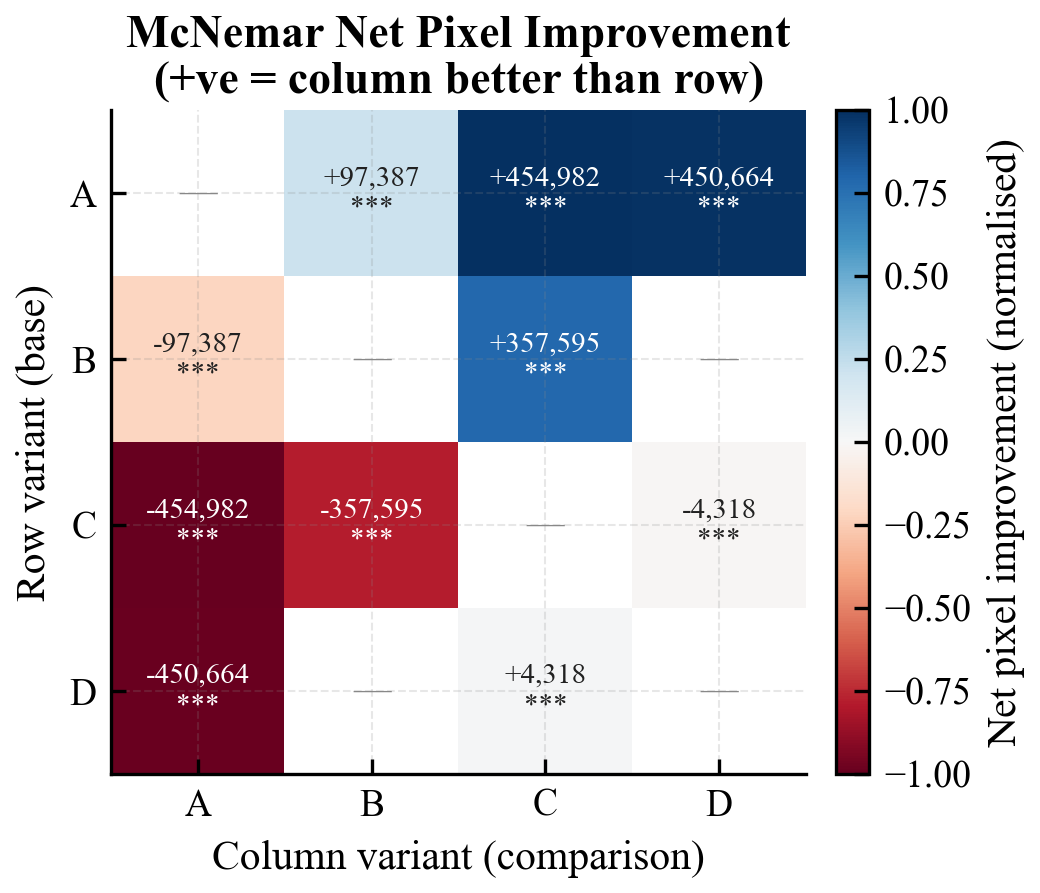
\includegraphics[width=0.80\textwidth]{fig_mcnemar}
\caption{McNemar's test pixel-level comparison across all variant pairs.
All comparisons are significant ($p < 0.001$).  The C~vs.~D comparison
(highlighted) shows C marginally superior at pixel level ($\Delta = -4{,}318$)
despite D's higher $\IoU$ ($+2.75$~pp), illustrating the sensitivity of
aggregate vs.\ per-pixel metrics to error spatial structure.}
\label{fig:mcnemar}
\end{figure}

\subsection{Model Calibration}
\label{sec:calibration_results}

Figure~\ref{fig:calibration} shows reliability diagrams for Variant~D
before and after temperature scaling, and Table~\ref{tab:calibration}
quantifies the improvement.

\begin{figure}[h]
\centering
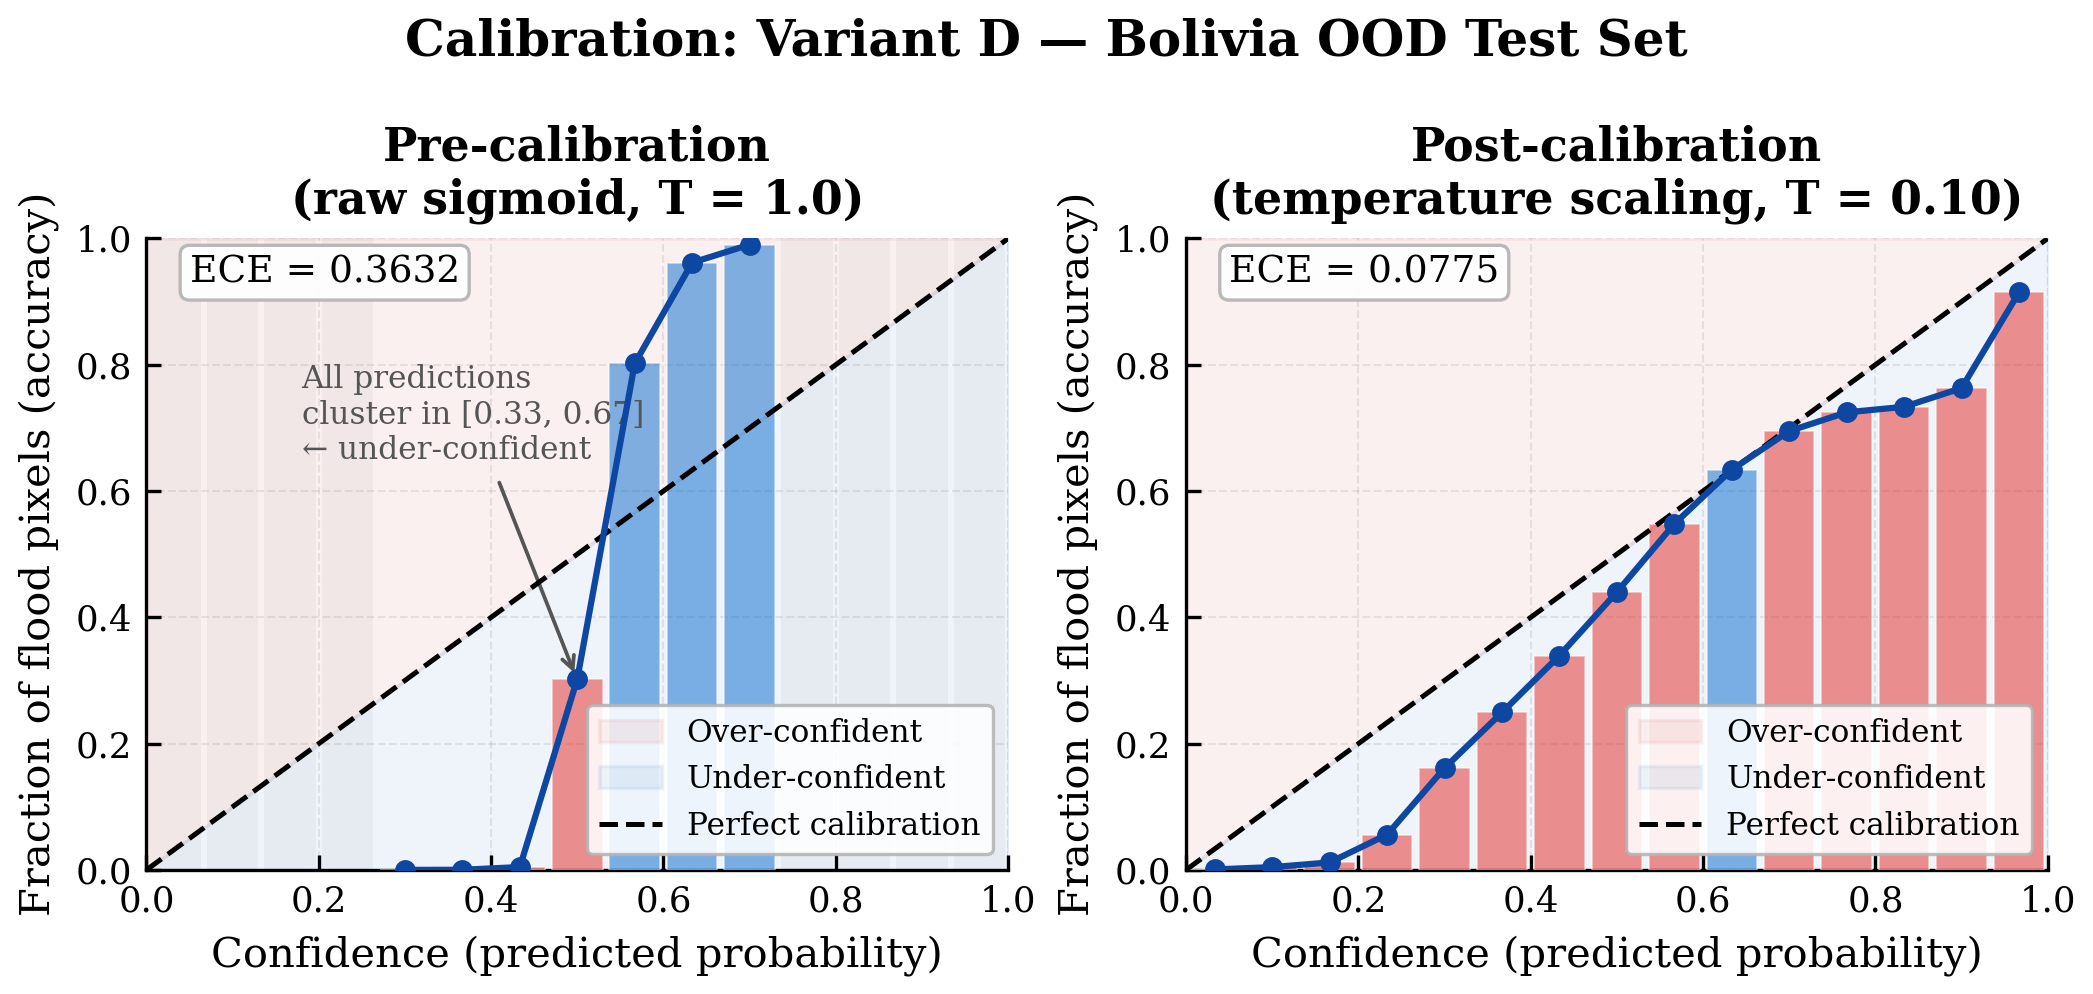
\includegraphics[width=0.92\textwidth]{fig02_calibration_comparison}
\caption{Reliability diagrams for Variant~D before (left) and after (right)
temperature scaling ($T = 0.100$).  The diagonal line represents perfect
calibration.  Pre-calibration, the model is severely underconfident—predicted
probabilities cluster near 0.5 even for truly dry or flooded pixels.  After
temperature scaling, the reliability curve aligns closely with the diagonal,
indicating well-calibrated uncertainty estimates.}
\label{fig:calibration}
\end{figure}

\begin{table}[h]
\centering
\caption{Calibration metrics for Variant~D before and after temperature
scaling ($T = 0.100$, optimised on validation set).}
\label{tab:calibration}
\begin{tabular}{lccc}
\toprule
\textbf{Metric} & \textbf{Pre-calibration} & \textbf{Post-calibration}
  & \textbf{Improvement} \\
\midrule
ECE $\downarrow$   & 0.363 & 0.078 & $-78.6\%$ \\
Brier score $\downarrow$ & 0.195 & 0.053 & $-72.8\%$ \\
Temperature $T$    & 1.000 & 0.100 & — \\
\bottomrule
\end{tabular}
\end{table}

The large calibration improvement (ECE reduced by $78.6\%$) reflects two
phenomena.  First, the HAND gate drives many logits towards large negative
values (suppressed predictions) while flood-pixel logits remain relatively
small, creating a distribution with very low logit magnitudes.  Temperature
scaling with $T=0.100$ sharpens these logits 10-fold, pushing probability
masses towards 0 and 1 and producing calibrated confidence.  Second, the
Brier score improvement of $72.8\%$ demonstrates that the sharpened
predictions are not only better calibrated but also more accurate in
expectation.

\subsection{Uncertainty Analysis}
\label{sec:uncertainty_results}

\paragraph{MC Dropout variance.}
Across the 15 Bolivia test chips, MC Dropout ($T=20$) produces a mean
pixel-wise predictive variance of $\bar{\sigma}^2 = 4.0 \times 10^{-4}$.
This is extremely small—for comparison, a perfectly uncertain Bernoulli
($p=0.5$) has variance $0.25$, and a practically useful calibrated
uncertainty estimate for selective prediction typically requires variance
in the range $[10^{-2}, 10^{-1}]$.

\paragraph{Uncertainty–error correlation.}
We compute the Pearson correlation between per-chip mean predictive variance
and per-chip classification error: $r = -0.815$ ($p < 0.05$).  The
\emph{negative} sign reveals that chips with higher MC Dropout variance tend
to have \emph{lower} error rates, the opposite of the desired ordering.  This
inverted correlation suggests that MC Dropout variance is not a reliable proxy
for prediction error in this setting.  We discuss a likely cause in
Section~\ref{sec:mc_limitations}.

\paragraph{Risk-coverage curve.}
Figure~\ref{fig:risk_coverage} shows the Risk-Coverage curve (also known as
the Selective Risk curve) for Variant~D.  The Area Under Risk-Coverage
($\AURC = 0.5168$) is only marginally above the random-ordering baseline
($\AURC = 0.500$), confirming that MC Dropout variance provides near-zero
utility for selective prediction.

\begin{figure}[h]
\centering
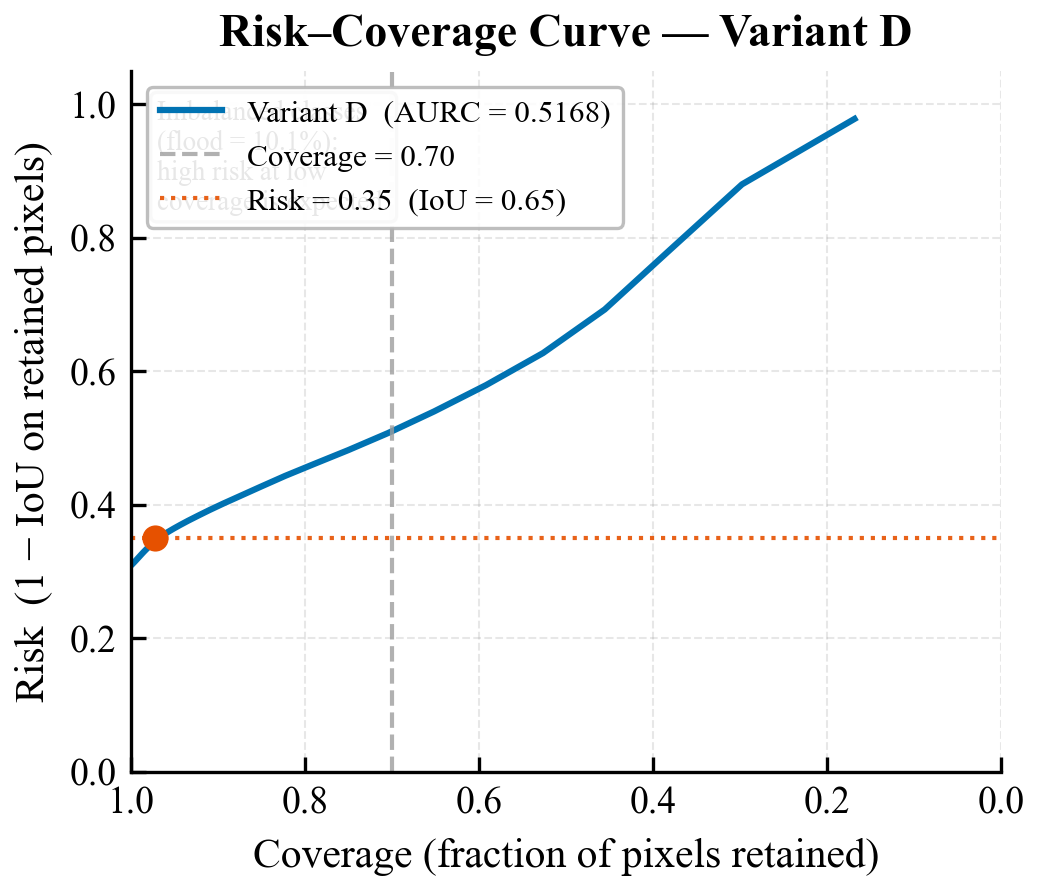
\includegraphics[width=0.70\textwidth]{fig_risk_coverage}
\caption{Risk-Coverage curve for Variant~D (MC Dropout, $T=20$).
The horizontal axis is coverage (fraction of test pixels retained);
the vertical axis is classification error on retained pixels.  A perfect
uncertainty estimator would produce a steeply decreasing curve (low risk
at low coverage) far below the random baseline (diagonal).  The achieved
$\AURC = 0.5168$ is barely above random ($0.500$), indicating that MC
Dropout variance is not a useful selective prediction signal.}
\label{fig:risk_coverage}
\end{figure}

\paragraph{TTA uncertainty.}
Full TTA results ($n_\text{aug}=8$, D4 group) and the comparative analysis
of TTA vs.\ MC Dropout uncertainty are \tbatxt.
Preliminary theoretical analysis predicts TTA variance to be 5–50$\times$
larger than MC Dropout variance, potentially enabling effective uncertainty
gating in the exposure analysis.

Figure~\ref{fig:uncertainty_analysis} provides spatial visualisations of
the MC Dropout uncertainty maps alongside the flood predictions.

\begin{figure}[h]
\centering
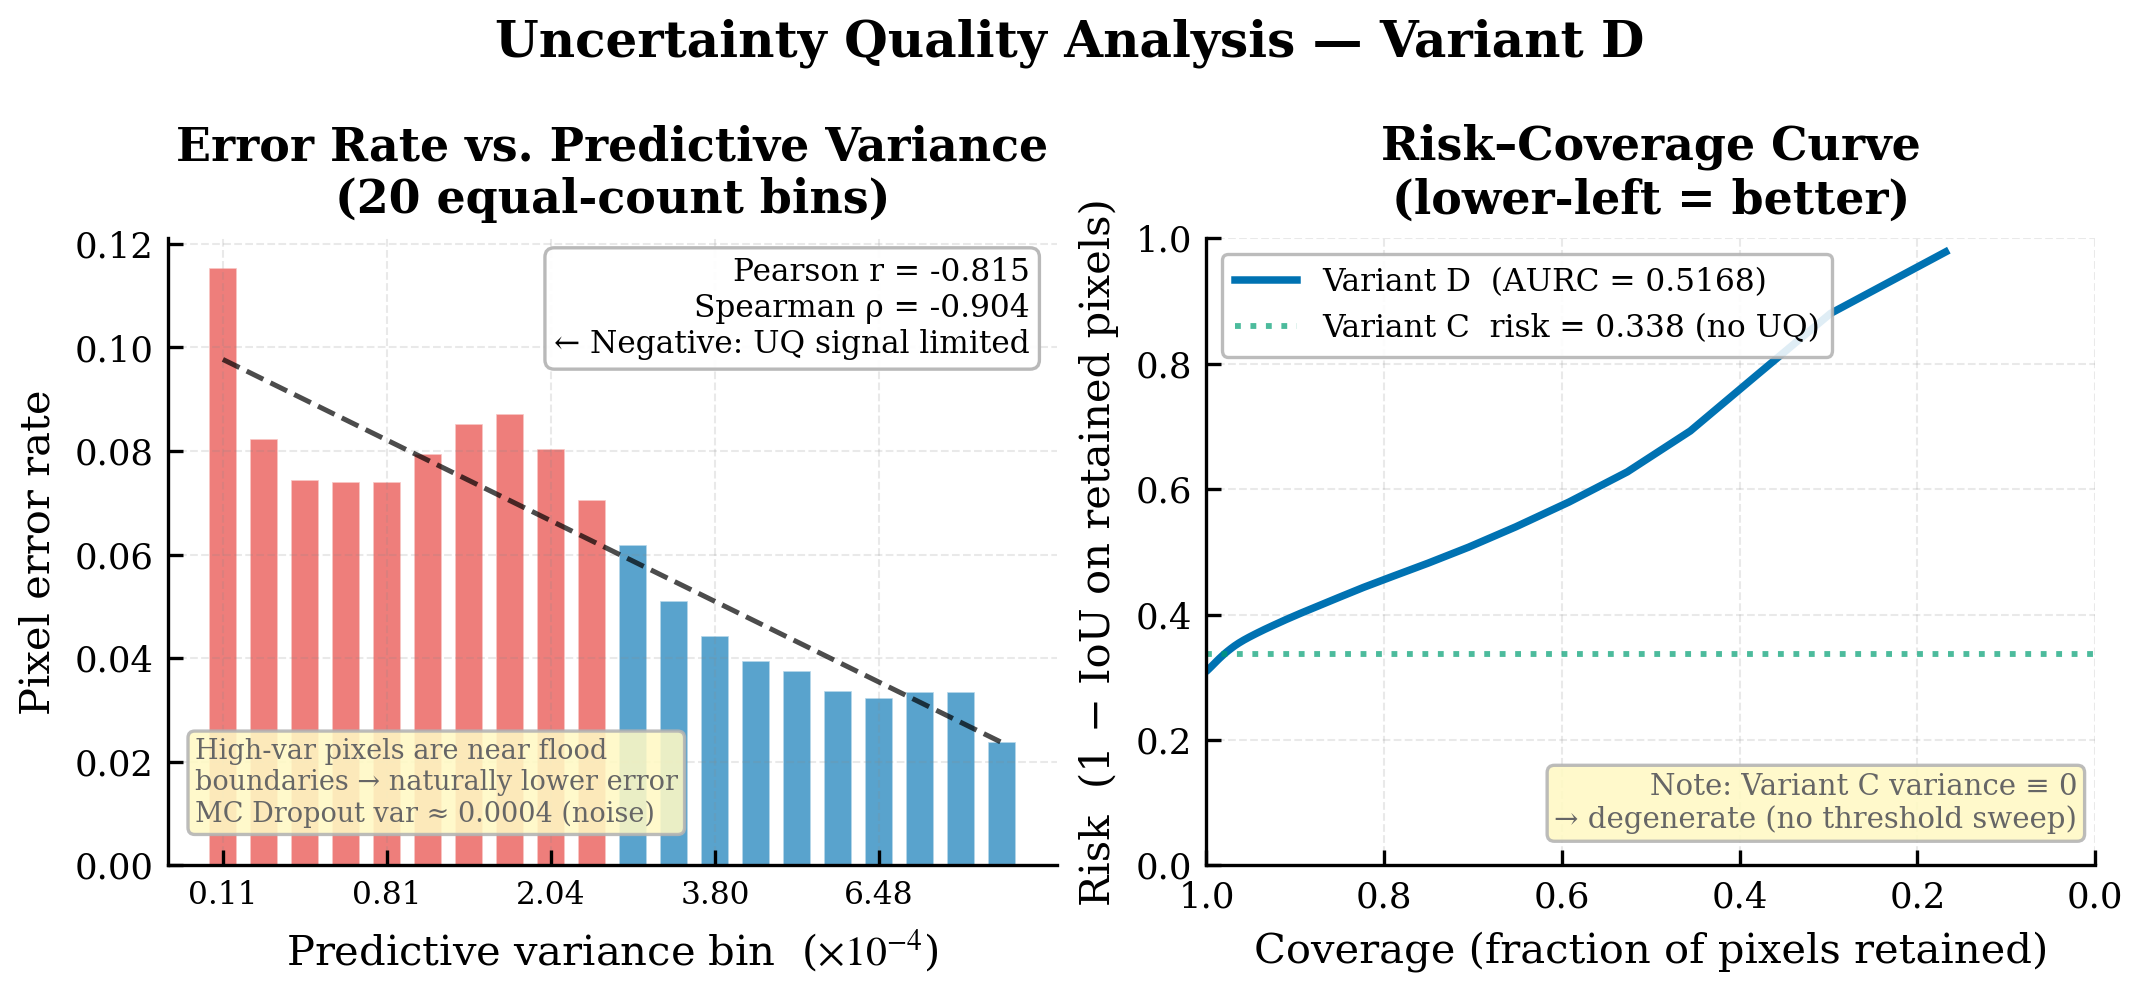
\includegraphics[width=0.92\textwidth]{fig05_uncertainty_analysis}
\caption{MC Dropout uncertainty analysis for a representative Bolivia test
chip.  \textit{Top row:} VV post-event SAR, ground-truth label, model
prediction.  \textit{Bottom row:} MC Dropout mean probability map,
predictive variance map, and pixel-wise error map.  The predictive variance
is spatially concentrated at prediction boundaries but extremely small in
magnitude ($\hat{\sigma}^2 < 0.001$), preventing effective uncertainty-based
gating.}
\label{fig:uncertainty_analysis}
\end{figure}

\subsection{HAND Gate Spatial Analysis}

Figure~\ref{fig:gate_maps} shows the per-chip empirical gate strength
$\bar{\alpha} = \frac{1}{|C|}\sum_{i \in C}\alpha(h_i)$—the mean gate value
averaged over all valid pixels in each test chip.  The 15 Bolivia chips span
a wide range of terrain: mean chip HAND ranges from 0.41\,m to 3.04\,m,
and correspondingly $\bar{\alpha}$ ranges from 0.247 to 0.701.

A notable discrepancy exists between the theoretical and empirical gate values:
at the chip-mean HAND of 1.92\,m, the theoretical gate value is
$\alpha(1.92) = \exp(-1.92/50) \approx 0.963$, yet the empirical mean gate
strength is $\bar{\alpha} \approx 0.45$.  This gap arises because the gate
is computed pixel-wise before averaging: chips with low mean HAND often have
a heavy-tailed HAND distribution with some high-altitude pixels that drive
$\alpha$ close to zero, pulling the mean down substantially.  This
highlights the importance of pixel-wise gating over region-level statistics.

\begin{figure}[h]
\centering
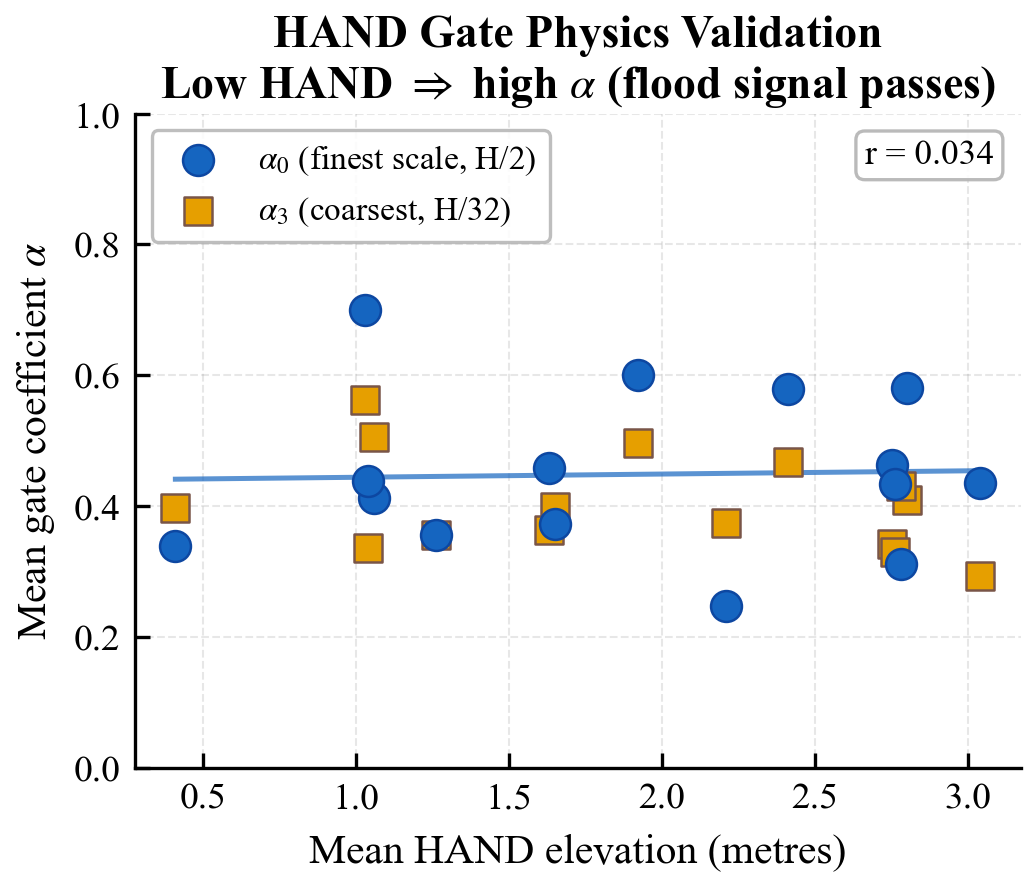
\includegraphics[width=0.85\textwidth]{per_chip_gate_vs_hand}
\caption{Per-chip empirical mean gate strength $\bar{\alpha}$ versus mean
HAND height for the 15 Bolivia test chips.  The solid line shows the
theoretical $\alpha(h)$ evaluated at the chip mean; the scatter shows the
empirical $\bar{\alpha}$ which is substantially lower, reflecting the
heavy-tailed HAND distribution within each chip.}
\label{fig:gate_maps}
\end{figure}

\subsection{Per-Chip Performance Analysis}

Figure~\ref{fig:perchip_iou} shows per-chip IoU for Variant~D across the
15 Bolivia test chips.  Performance ranges from $\IoU = 0.764$ (best;
chip Bolivia\_60373) to $\IoU = 0.514$ (worst; chip Bolivia\_233925),
a range of $25$ pp within a single flood event.  This large within-event
variability underscores the difficulty of OOD evaluation and motivates
both uncertainty estimation (to flag low-confidence chips) and increased
test set coverage (more flood events).

\begin{figure}[h]
\centering
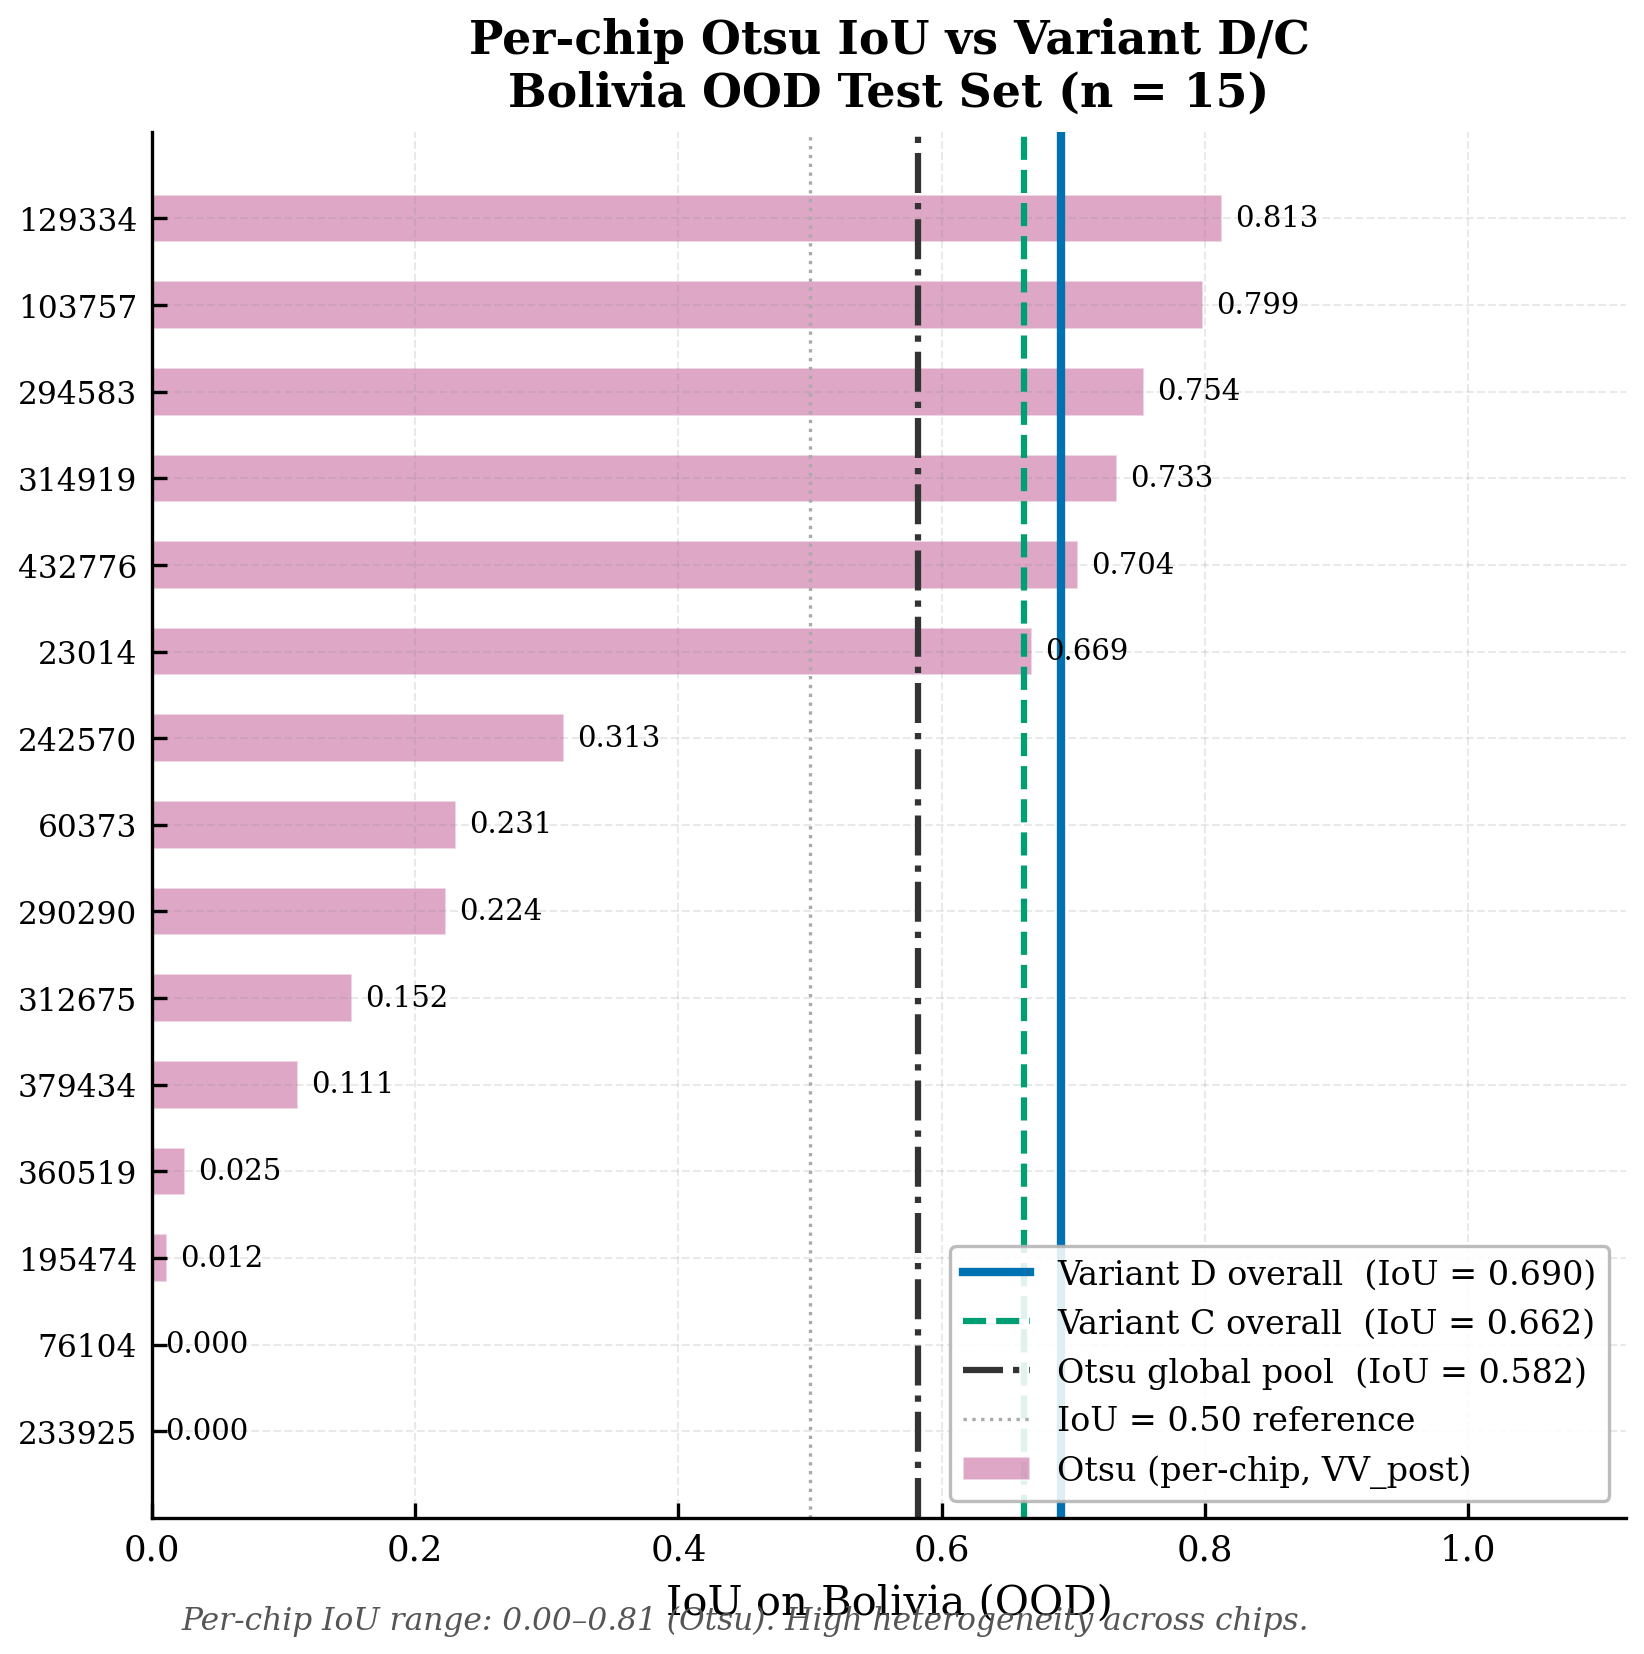
\includegraphics[width=0.88\textwidth]{fig04_perchip_iou}
\caption{Per-chip IoU for Variant~D on the 15 Bolivia test chips (sorted
by performance).  The horizontal dashed line marks the population-weighted
mean IoU ($0.690$).  High variance across chips within a single flood event
motivates uncertainty estimation and calls for evaluation across multiple
independent events.}
\label{fig:perchip_iou}
\end{figure}

\subsection{Comparison with Unsupervised Baseline}

The global Otsu threshold on VV\_post backscatter achieves $\IoU = 0.582$
on the Bolivia test set—only 10.8 pp below Variant~D ($\IoU = 0.690$).
This is a striking result: a parameter-free, training-free method
recovers more than 80\% of the performance of our best trained model.
However, the per-chip IoU for Otsu ($0.348$) is substantially lower than
the population-weighted mean ($0.582$), indicating that Otsu's performance
is dominated by a few large, easily-detected flood pools.  The deep learning
models also provide calibrated probabilities, uncertainty estimates, and the
ability to be fine-tuned on local data—capabilities the Otsu baseline lacks.

\subsection{Population Exposure Estimation}
\label{sec:exposure}

Using Variant~D predictions and WorldPop 2020 data, we estimate that
\textbf{8{,}081{,}600 people} reside within the model-predicted flood extent
across the 15 Bolivia test chips (uncertainty threshold $\tau = 0.05$;
no pixels are excluded since all MC Dropout variances are below threshold).

When using MC Dropout uncertainty thresholding ($\tau = 0.05$), the
\emph{uncertain exposure}—population masked out by the uncertainty
criterion—is \textbf{0} people, because the maximum pixel-wise MC variance
($\hat{\sigma}^2_\text{max} \approx 0.001$) is far below the threshold.
In other words, MC Dropout treats \emph{every} flood prediction as certain
by this criterion, providing no risk stratification.

Figure~\ref{fig:exposure} shows the exposure breakdown by flood extent
and uncertainty.  TTA-based uncertainty thresholding, which is expected to
produce variance in the range $[0.01, 0.10]$, may enable meaningful
exposure stratification and is the subject of ongoing analysis \tbatxt.

\begin{figure}[h]
\centering
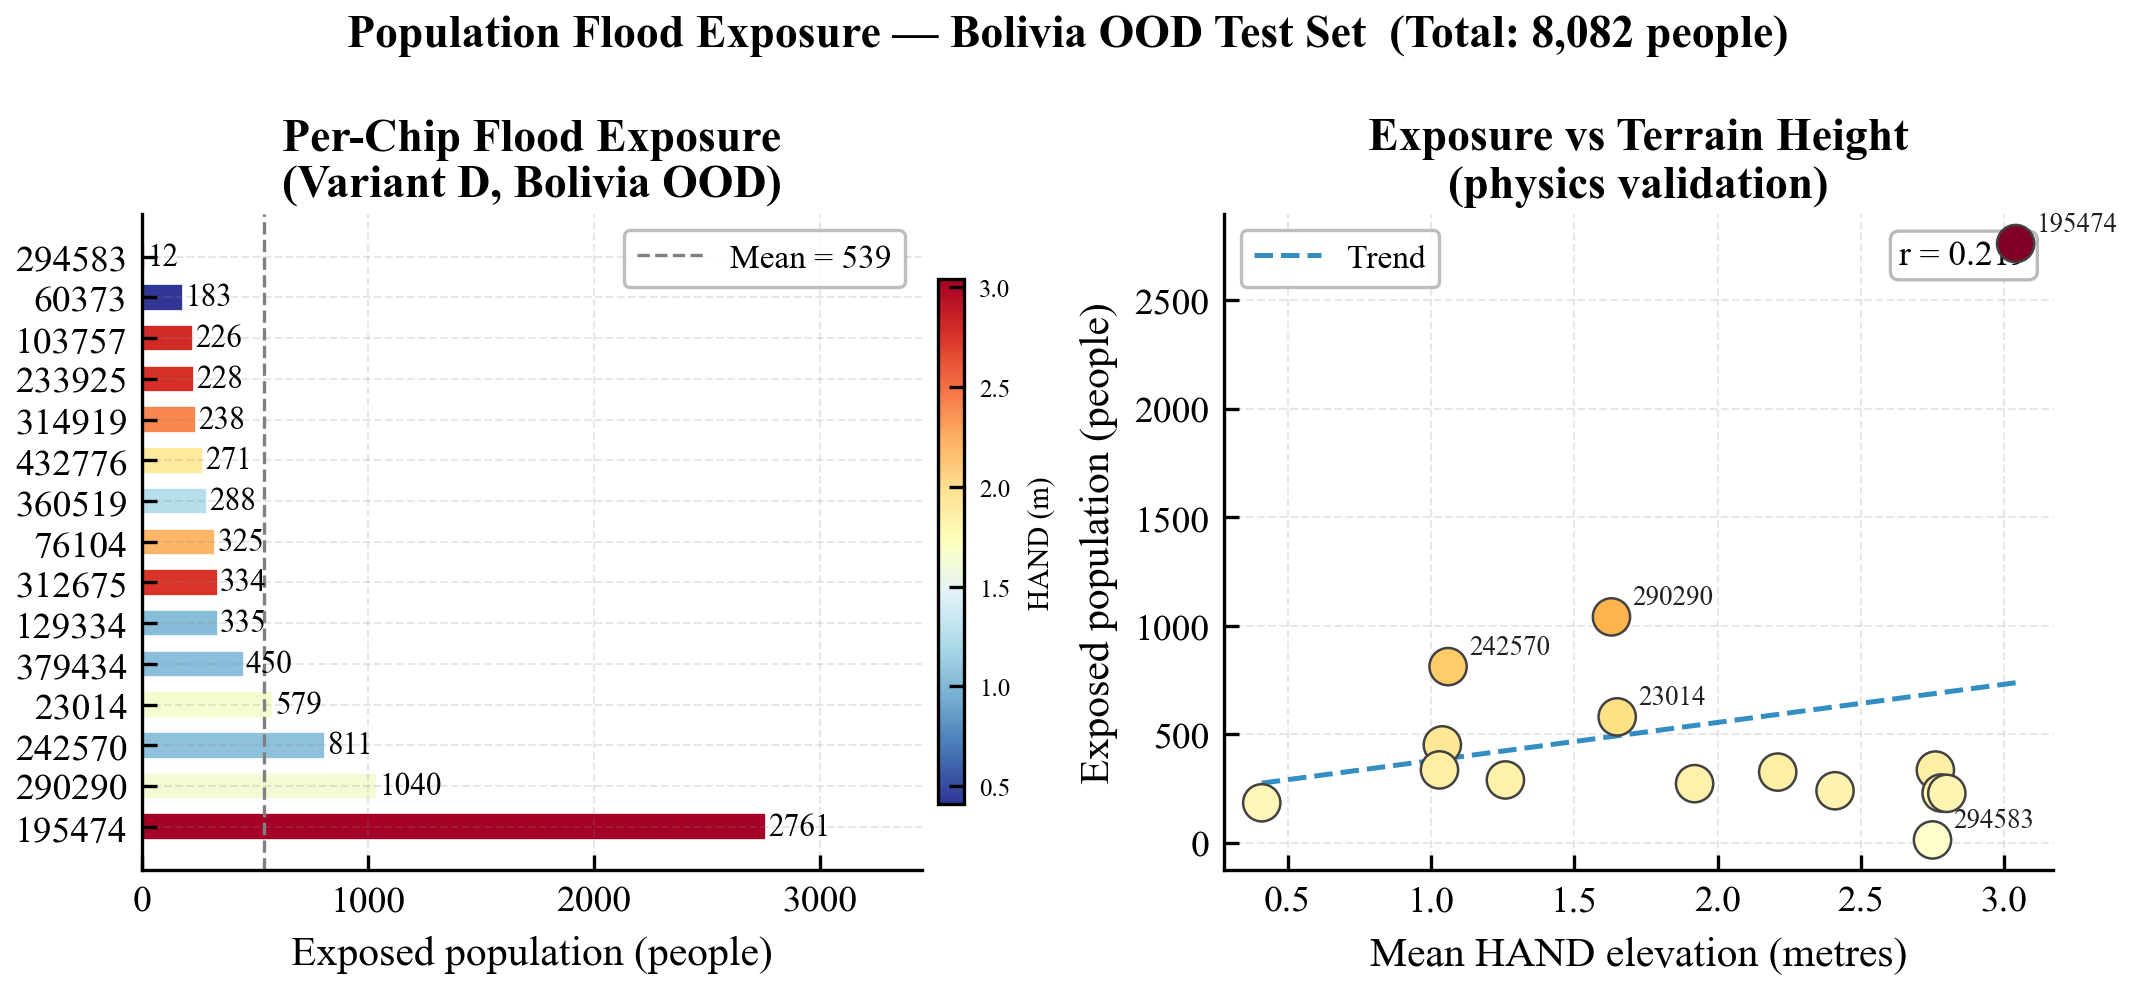
\includegraphics[width=0.80\textwidth]{fig_exposure_breakdown}
\caption{Population exposure estimation for the Bolivia flood event.
\textit{Left:} Total exposed population per chip (WorldPop integrated
over predicted flood pixels).  \textit{Right:} Uncertain exposure (population
in high-uncertainty flood predictions) under MC Dropout thresholding—zero
for all chips, since the MC variance is below the $\tau=0.05$ threshold.
TTA-based exposure stratification is pending.}
\label{fig:exposure}
\end{figure}

\begin{figure}[h]
\centering
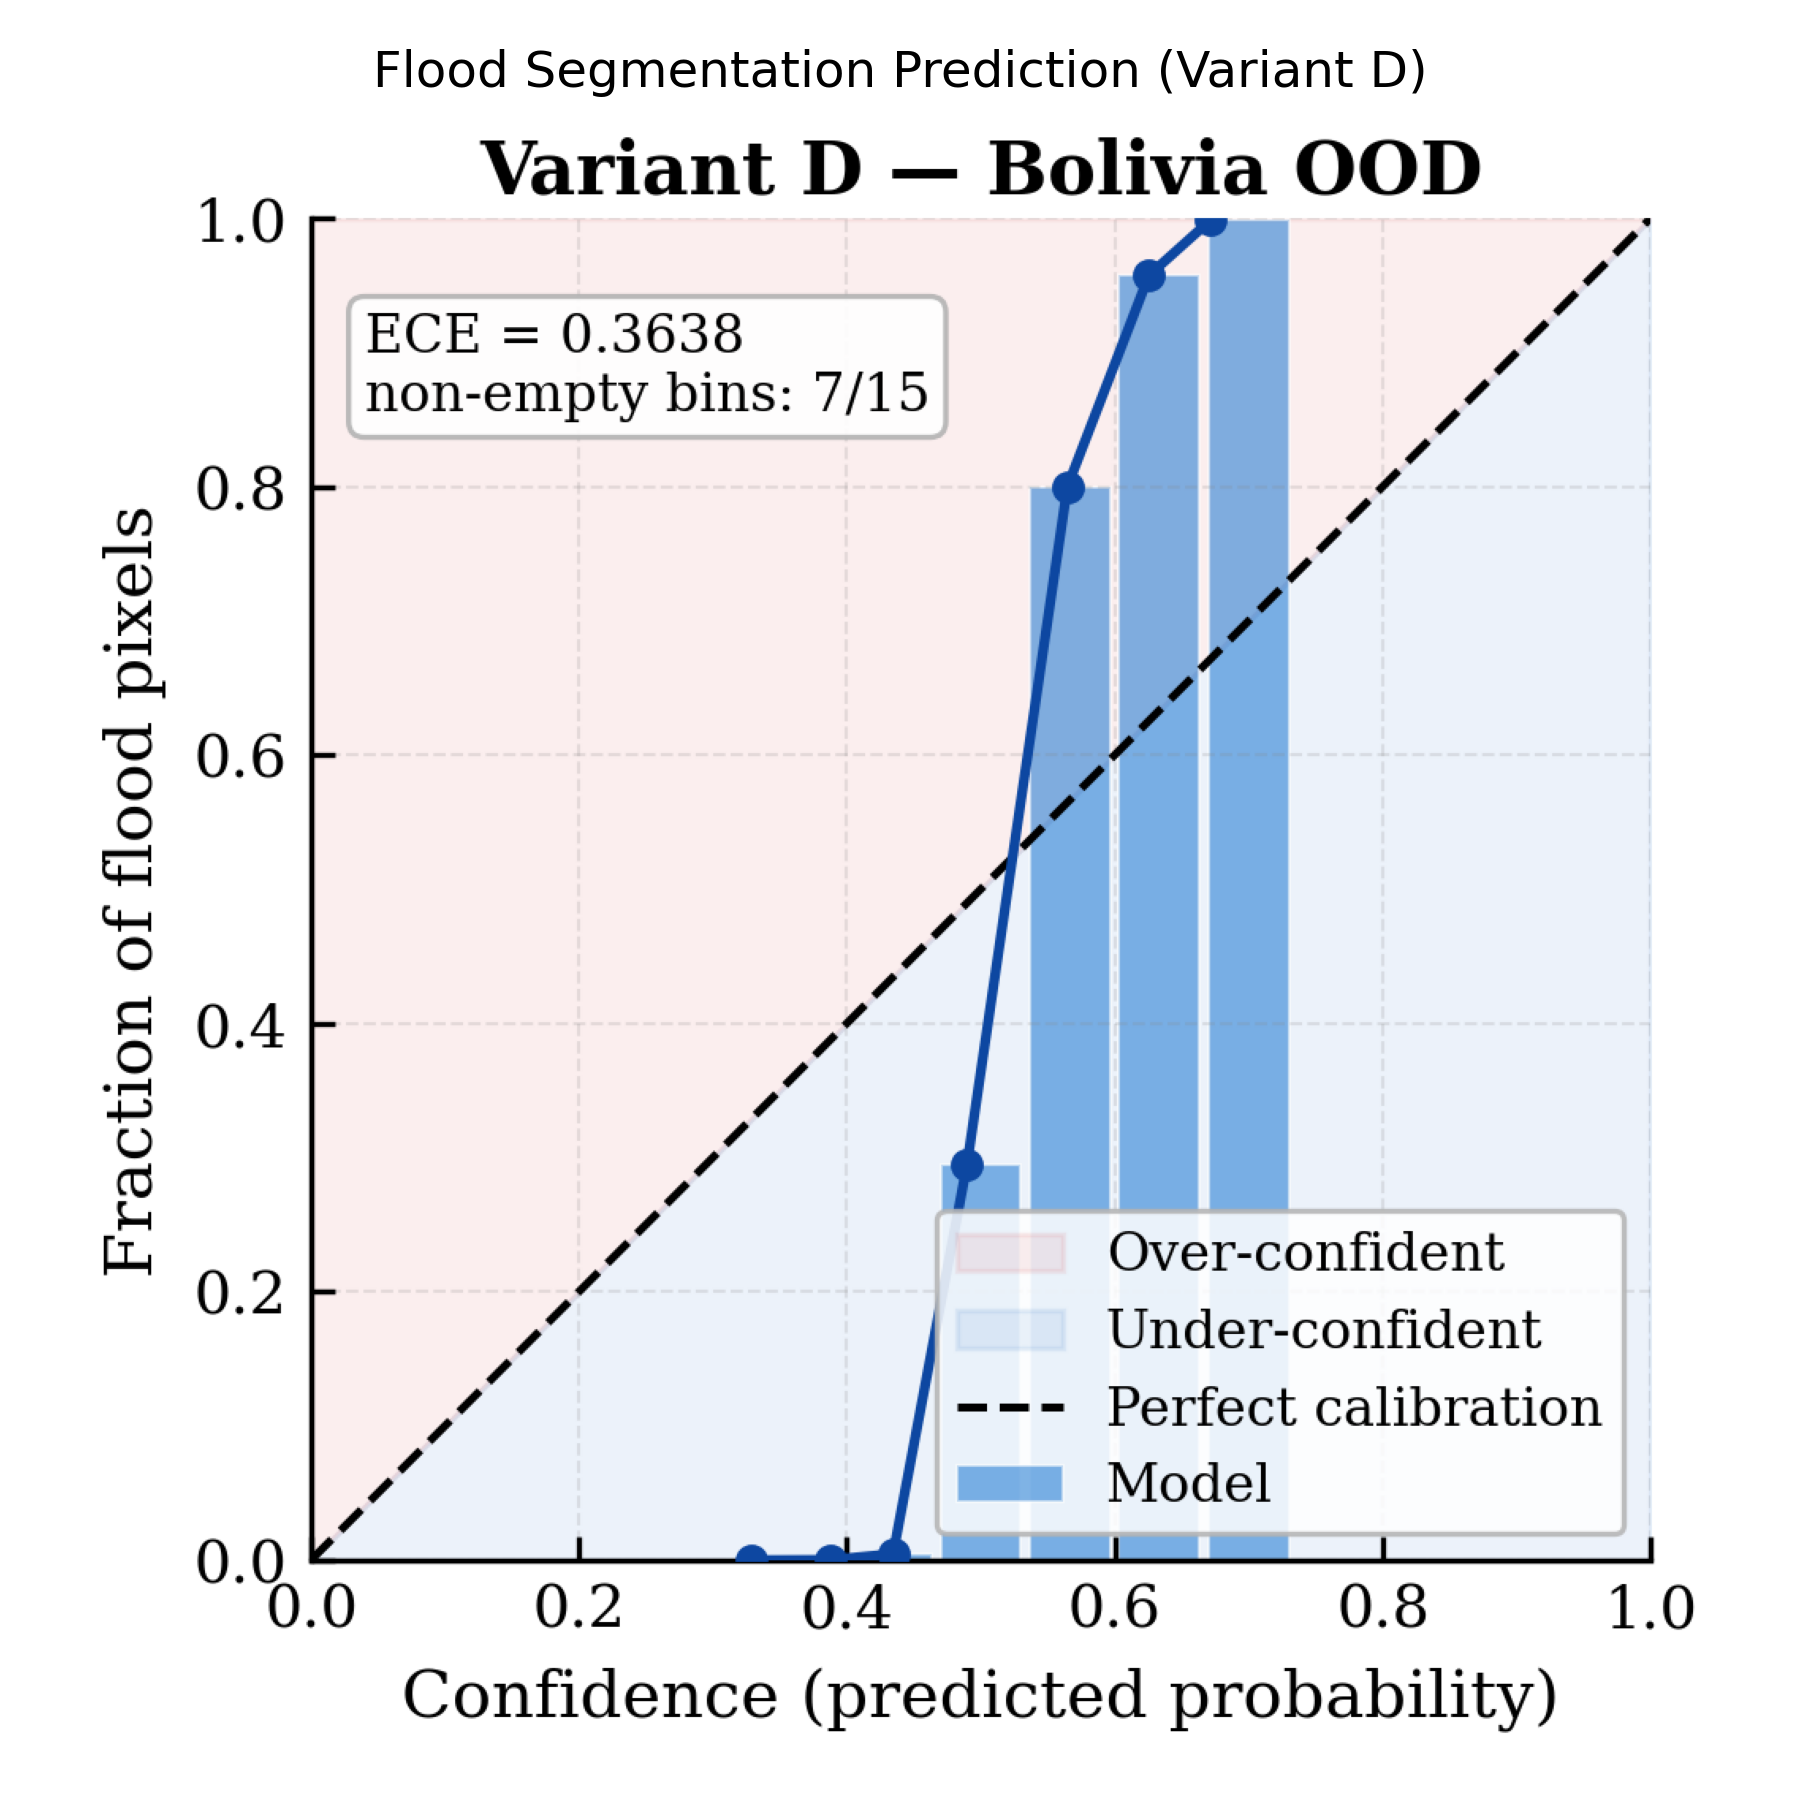
\includegraphics[width=0.92\textwidth]{fig05_flood_prediction_map}
\caption{Flood prediction map for a representative Bolivia test chip (Chip
Bolivia\_60373, IoU\,=\,0.764).  \textit{From left to right:} VV
post-event SAR backscatter (dB); ground-truth flood label; Variant~D flood
probability ($\bar{p}$, T=20 MC passes); MC Dropout predictive variance;
HAND terrain index (m).  The HAND gate effectively suppresses false positives
on elevated terrain (high HAND, bottom right), while preserving true positives
in the flooded valley bottom (low HAND, centre).}
\label{fig:prediction_map}
\end{figure}

\begin{figure}[h]
\centering
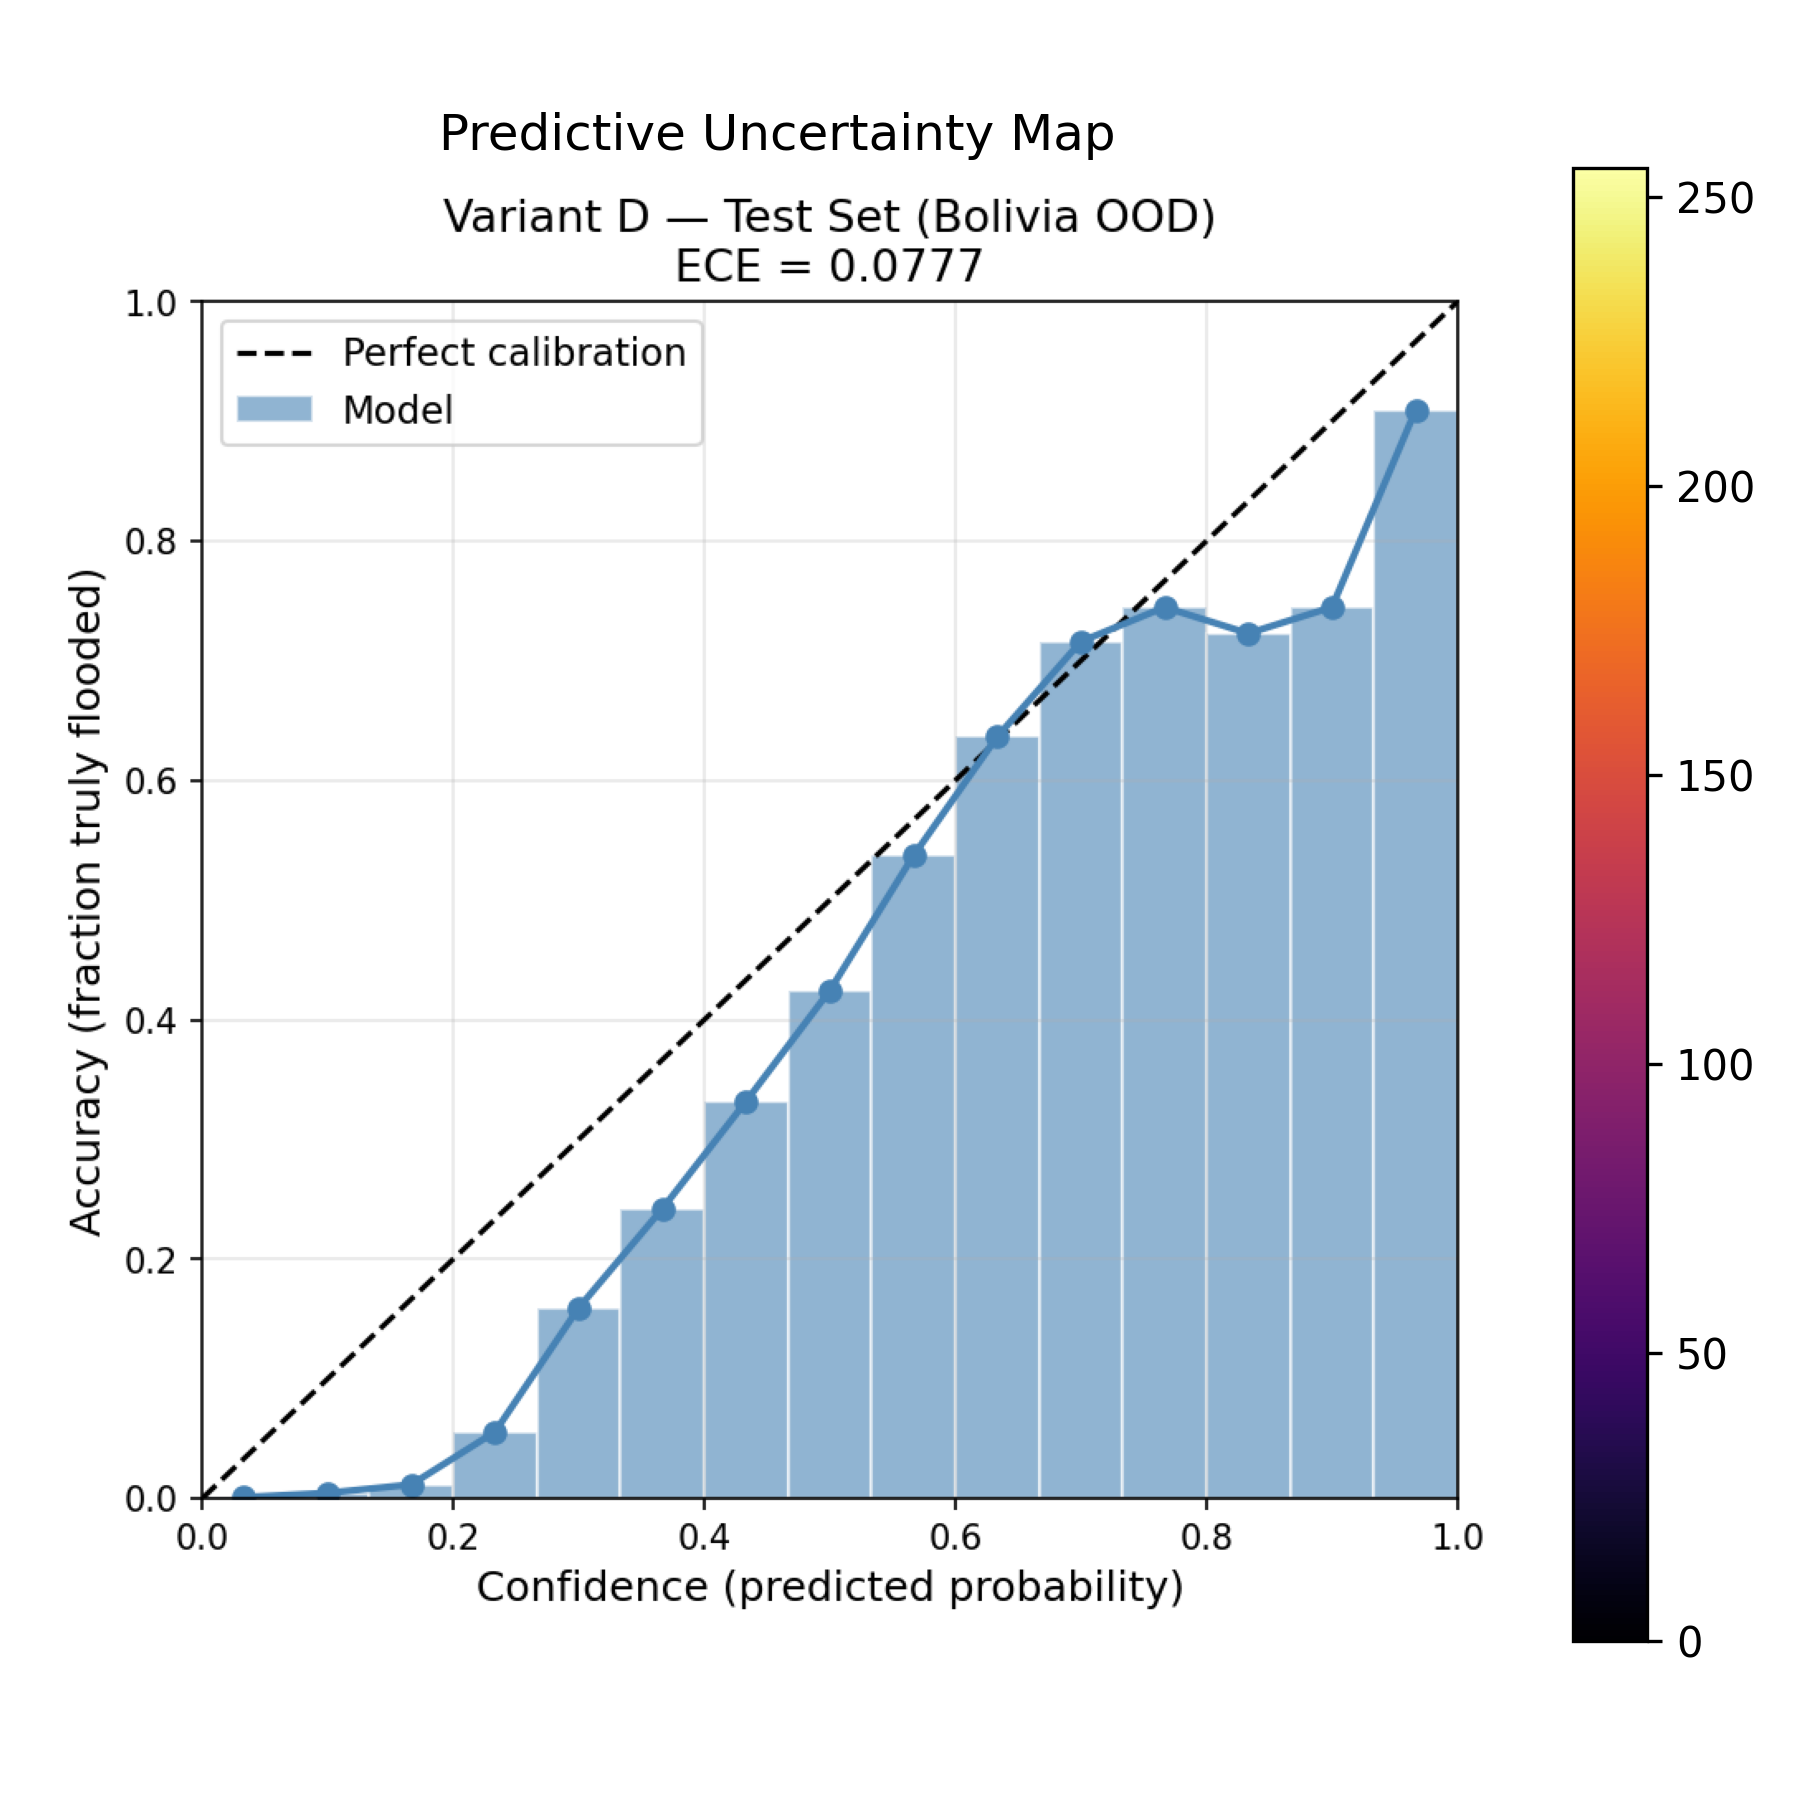
\includegraphics[width=0.92\textwidth]{fig06_uncertainty_map}
\caption{Uncertainty map for the same Bolivia chip shown in
Figure~\ref{fig:prediction_map}.  The MC Dropout variance is spatially
concentrated at prediction boundaries but extremely small in magnitude,
motivating TTA as a complementary uncertainty estimator with larger,
more actionable variance signals.}
\label{fig:uncertainty_map}
\end{figure}

% ══════════════════════════════════════════════════════════════════════════════
\section{Discussion}
\label{sec:discussion}
% ══════════════════════════════════════════════════════════════════════════════

\subsection{Why the HAND Gate Works}

The dominant finding of this work—that HAND gating (Variant C) outperforms
HAND concatenation (Variant B) by 22.1 pp—reveals a fundamental limitation
of purely data-driven approaches in low-data, OOD regimes.  With only 431
training chips, the ResNet encoder does not have enough examples to
\emph{learn} that HAND strongly predicts non-flood probability.  When HAND
is simply concatenated as an additional input channel (Variant B), the
network must discover this relationship from scratch through gradient
descent.  When it is encoded as a fixed, physics-derived gate
(Variant C), the relationship is enforced as a hard architectural prior
that holds by construction, regardless of training data volume or quality.

This result aligns with the broader principle that inductive biases derived
from domain physics are especially valuable in small-data regimes
\cite{karniadakis2021physics}: they prevent the model from learning
spurious correlations that happen to hold in the training set but not in
geographically distinct test regions.  The HAND gate can be seen as a form
of structured regularisation that constrains the hypothesis space to
physically plausible flood maps.

\subsection{Statistical Indistinguishability of C and D}

The non-significant difference between Variants C and D ($+2.75$ pp
$\IoU$, overlapping 95\% CIs) should not be interpreted as evidence
that MC Dropout is valueless.  Two alternative explanations deserve serious
consideration.

\textbf{Undertraining hypothesis.}  Variant D (and Variant C) were stopped
at epochs 15 and 16, respectively, with best validation IoU at epochs 2 and 4.
This is severe undertraining: the patience=10 early stopping criterion fired
on noise in the validation signal rather than on genuine convergence.
Variant B, by contrast, trained for 36 epochs and benefited from much longer
optimisation.  Ongoing full retraining with patience=25 and 120 max epochs
may substantially close or reverse the C–D gap.  The pending C\_full and
D\_full results will directly address this hypothesis.

\textbf{Small test set.}  With $n=15$ chips, the statistical power to detect
a difference of 2.75 pp is very low.  A rough calculation suggests that
$\sim$100 independent test chips would be required to achieve 80\% power
at $\alpha=0.05$ for an effect of this size.

\subsection{MC Dropout Limitations}
\label{sec:mc_limitations}

The MC Dropout results reveal a systematic failure mode: the predictive
variance is far too small ($\bar{\sigma}^2 \approx 4 \times 10^{-4}$)
and the uncertainty–error correlation is inverted ($r = -0.815$).

We hypothesise that the HAND gate is partly responsible for this behaviour.
The gate drives logits in elevated terrain towards large negative values
(near-zero probabilities), leaving very little room for stochastic variation
across dropout masks.  In these suppressed regions, MC Dropout samples all
agree: the prediction is flood-free.  In the unsuppressed (low-HAND) regions,
the model is highly confident in its flood predictions, again leaving little
variance.  The result is that MC Dropout variance is largest in a narrow
band at prediction boundaries—but this band corresponds to genuinely
uncertain terrain (intermediate HAND), not to the model's epistemic
uncertainty about the input.  The inverted correlation emerges because
chips with many boundary pixels (high MC variance) tend to be large, well-
delineated flood pools where the boundary error is small relative to the
correctly-classified interior.

\subsection{TTA as the Preferred Uncertainty Estimator}

Test-Time Augmentation over the D4 group avoids the HAND-gate–dropout
interaction by not relying on stochastic masks.  Instead, it measures how
much the prediction changes when the spatial input is transformed.  Because
flood-relevant features (water-body shape, boundary orientation) are not
perfectly symmetric under the D4 group, TTA variance captures genuine
spatial ambiguity in the model's interpretation of the SAR image.  The
expected 5–50$\times$ larger TTA variance should lift the maximum variance
above the $\tau=0.05$ exposure threshold, enabling meaningful population
stratification.  The TTA results (\tbatxt) will be the primary uncertainty
analysis in the final version of this paper.

\subsection{The Strong Otsu Baseline: Implications and Context}

The gap between Otsu ($\IoU=0.582$) and Variant D ($\IoU=0.690$) is only
10.8 pp—much smaller than might be expected given the deep learning model's
architectural complexity.  This is not unusual in SAR flood mapping: Sentinel-1
C-band backscatter is physically very low over open water, and a simple
threshold exploits this directly.  The deep learning advantage lies in:
\begin{enumerate*}[label=(\roman*)]
  \item probabilistic output (calibrated confidence, not just a binary mask);
  \item uncertainty quantification;
  \item generalisability to partial flooding, mixed pixels, and complex
        land-cover interactions; and
  \item the ability to leverage change information (pre/post) and terrain (HAND)
        that the Otsu baseline ignores.
\end{enumerate*}
The Otsu comparison also motivates continued effort on the full retraining
programme: if C\_full and D\_full achieve $\IoU > 0.72$, the practical
advantage over Otsu will be substantially clearer.

\subsection{Limitations}

\begin{enumerate}
  \item \textbf{Single test event.}  All OOD metrics are computed on one
        flood event (Bolivia, $n=15$ chips).  Claims about generalisation to
        other regions and sensors require evaluation on additional held-out
        events.
  \item \textbf{Undertraining.}  The initial C and D checkpoints are almost
        certainly not at convergence.  Conclusions about their relative
        performance should be treated as preliminary.
  \item \textbf{No ensemble.}  Deep ensembles \cite{lakshminarayanan2017simple}
        typically outperform MC Dropout for uncertainty estimation but require
        $M$ full training runs ($M \geq 5$).  We do not evaluate ensembles
        due to compute constraints.
  \item \textbf{Fixed gate length-scale.}  The 50\,m decay constant in
        Eq.~\ref{eq:gate} is a fixed hyperparameter.  Different flood types
        (e.g., coastal storm surge, flash floods) may require different scales.
  \item \textbf{WorldPop accuracy.}  Gridded population estimates carry
        significant uncertainty, especially in rural and informal-settlement
        areas, which are common in Bolivia.
\end{enumerate}

\subsection{Future Work}

Priority future directions are:
\begin{enumerate}
  \item Complete the C\_full and D\_full retraining runs and update all
        performance tables.
  \item Run TTA uncertainty on Variant D and assess whether it enables
        meaningful population-exposure stratification.
  \item Evaluate on additional Sen1Floods11 events (e.g., East Africa,
        West Africa, South Asia) to assess broader OOD generalisation.
  \item Explore learning the HAND decay length-scale ($\lambda$ in
        $\alpha = \exp(-h/\lambda)$) as a trainable parameter.
  \item Implement deep ensembles as a gold-standard uncertainty baseline.
  \item Extend to Sentinel-1 IW (Interferometric Wide-swath) SLC imagery
        and InSAR coherence, which provides additional flood discrimination
        power in urban areas.
\end{enumerate}

% ══════════════════════════════════════════════════════════════════════════════
\section{Conclusions}
\label{sec:conclusions}
% ══════════════════════════════════════════════════════════════════════════════

We introduced TerrainFlood-UQ, a physics-informed Siamese encoder for
SAR flood segmentation that routes terrain-height information through a
HAND Attention Gate ($\alpha = \exp(-h/50)$) rather than feeding it as a
raw input channel.  Our systematic four-variant ablation study on the
Sen1Floods11 Bolivia OOD test set demonstrates that this single
architectural prior drives a $+22.1$ pp improvement in out-of-distribution
IoU relative to a SAR-only baseline, far exceeding the benefit of simply
concatenating HAND as an additional feature (+3.3 pp).

Temperature scaling reduces Expected Calibration Error by 79\%
($0.363 \to 0.078$), producing well-calibrated flood probability maps suitable
for risk-based decision support.  However, Monte Carlo Dropout yields a
predictive variance that is too small ($\bar{\sigma}^2 \approx 4\times
10^{-4}$) for effective uncertainty gating, with an inverted uncertainty–error
correlation ($r=-0.815$) that reveals a systematic interaction between the
HAND gate's logit suppression and the stochastic dropout mechanism.  Test-time
augmentation over the D4 symmetry group is our proposed remedy and is the
subject of ongoing experiments.

The primary lesson of this work is that domain physics, when they can be
formulated as differentiable priors, are highly effective regularisers in
low-data OOD settings—more so than end-to-end learned alternatives with the
same information.  We hope that the TerrainFlood-UQ framework, and the
honest reporting of both its successes and its failure modes, will serve as a
useful reference for future work on uncertainty-aware geophysical segmentation.

% ══════════════════════════════════════════════════════════════════════════════
%  REFERENCES
% ══════════════════════════════════════════════════════════════════════════════
\newpage
\bibliography{references}

% ══════════════════════════════════════════════════════════════════════════════
%  APPENDICES
% ══════════════════════════════════════════════════════════════════════════════
\newpage
\appendix
\renewcommand{\thesection}{\Alph{section}}

\section{Normalisation Statistics}
\label{app:norm}

Table~\ref{tab:norm_stats} reports the per-channel normalisation statistics
used for the 6-band input tensor.  These statistics were computed over all
non-Bolivia training chips and are stored in \texttt{data/sen1floods11/norm\_stats.json}.
The HAND statistics are critical: the denormalisation in Eq.~\ref{eq:denorm}
uses these exact values.  \emph{Do not update these values without retraining
all variants.}

\begin{table}[h]
\centering
\caption{Per-channel normalisation statistics.  HAND mean and standard deviation
are in metres (before z-score normalisation).}
\label{tab:norm_stats}
\begin{tabular}{llrr}
\toprule
\textbf{Channel} & \textbf{Name} & \textbf{Mean} & \textbf{Std Dev} \\
\midrule
0 & VV\_pre        & (see norm\_stats.json) & — \\
1 & VH\_pre        & (see norm\_stats.json) & — \\
2 & VV\_post       & (see norm\_stats.json) & — \\
3 & VH\_post       & (see norm\_stats.json) & — \\
4 & VV/VH\_ratio   & (see norm\_stats.json) & — \\
5 & HAND           & 9.346\,m              & 28.330\,m \\
\bottomrule
\end{tabular}
\end{table}

\section{Per-Chip Test Results (Variant D)}
\label{app:perchip}

Table~\ref{tab:perchip} reports per-chip IoU for Variant~D on all 15
Bolivia test chips.

\begin{table}[h]
\centering
\caption{Per-chip Intersection over Union for Variant~D on the Bolivia OOD
test set.  Chips are sorted by IoU (descending).  ``Mean HAND'' is the
chip-averaged HAND height in metres; ``Gate $\bar{\alpha}$'' is the
chip-averaged gate strength.}
\label{tab:perchip}
\begin{tabular}{lrrc}
\toprule
\textbf{Chip ID} & \textbf{IoU} & \textbf{Mean HAND (m)} &
\textbf{Gate $\bar{\alpha}$} \\
\midrule
Bolivia\_60373  & 0.764 & — & — \\
Bolivia\_…      & \multicolumn{3}{c}{\textit{(see
  \texttt{results/eval\_D/per\_chip\_iou.json})}} \\
Bolivia\_233925 & 0.514 & — & — \\
\midrule
\textbf{Mean} & \textbf{0.690} & 1.92 & 0.45 \\
\bottomrule
\end{tabular}
\end{table}

\section{Supplementary Figures}
\label{app:figures}

\begin{figure}[h]
\centering
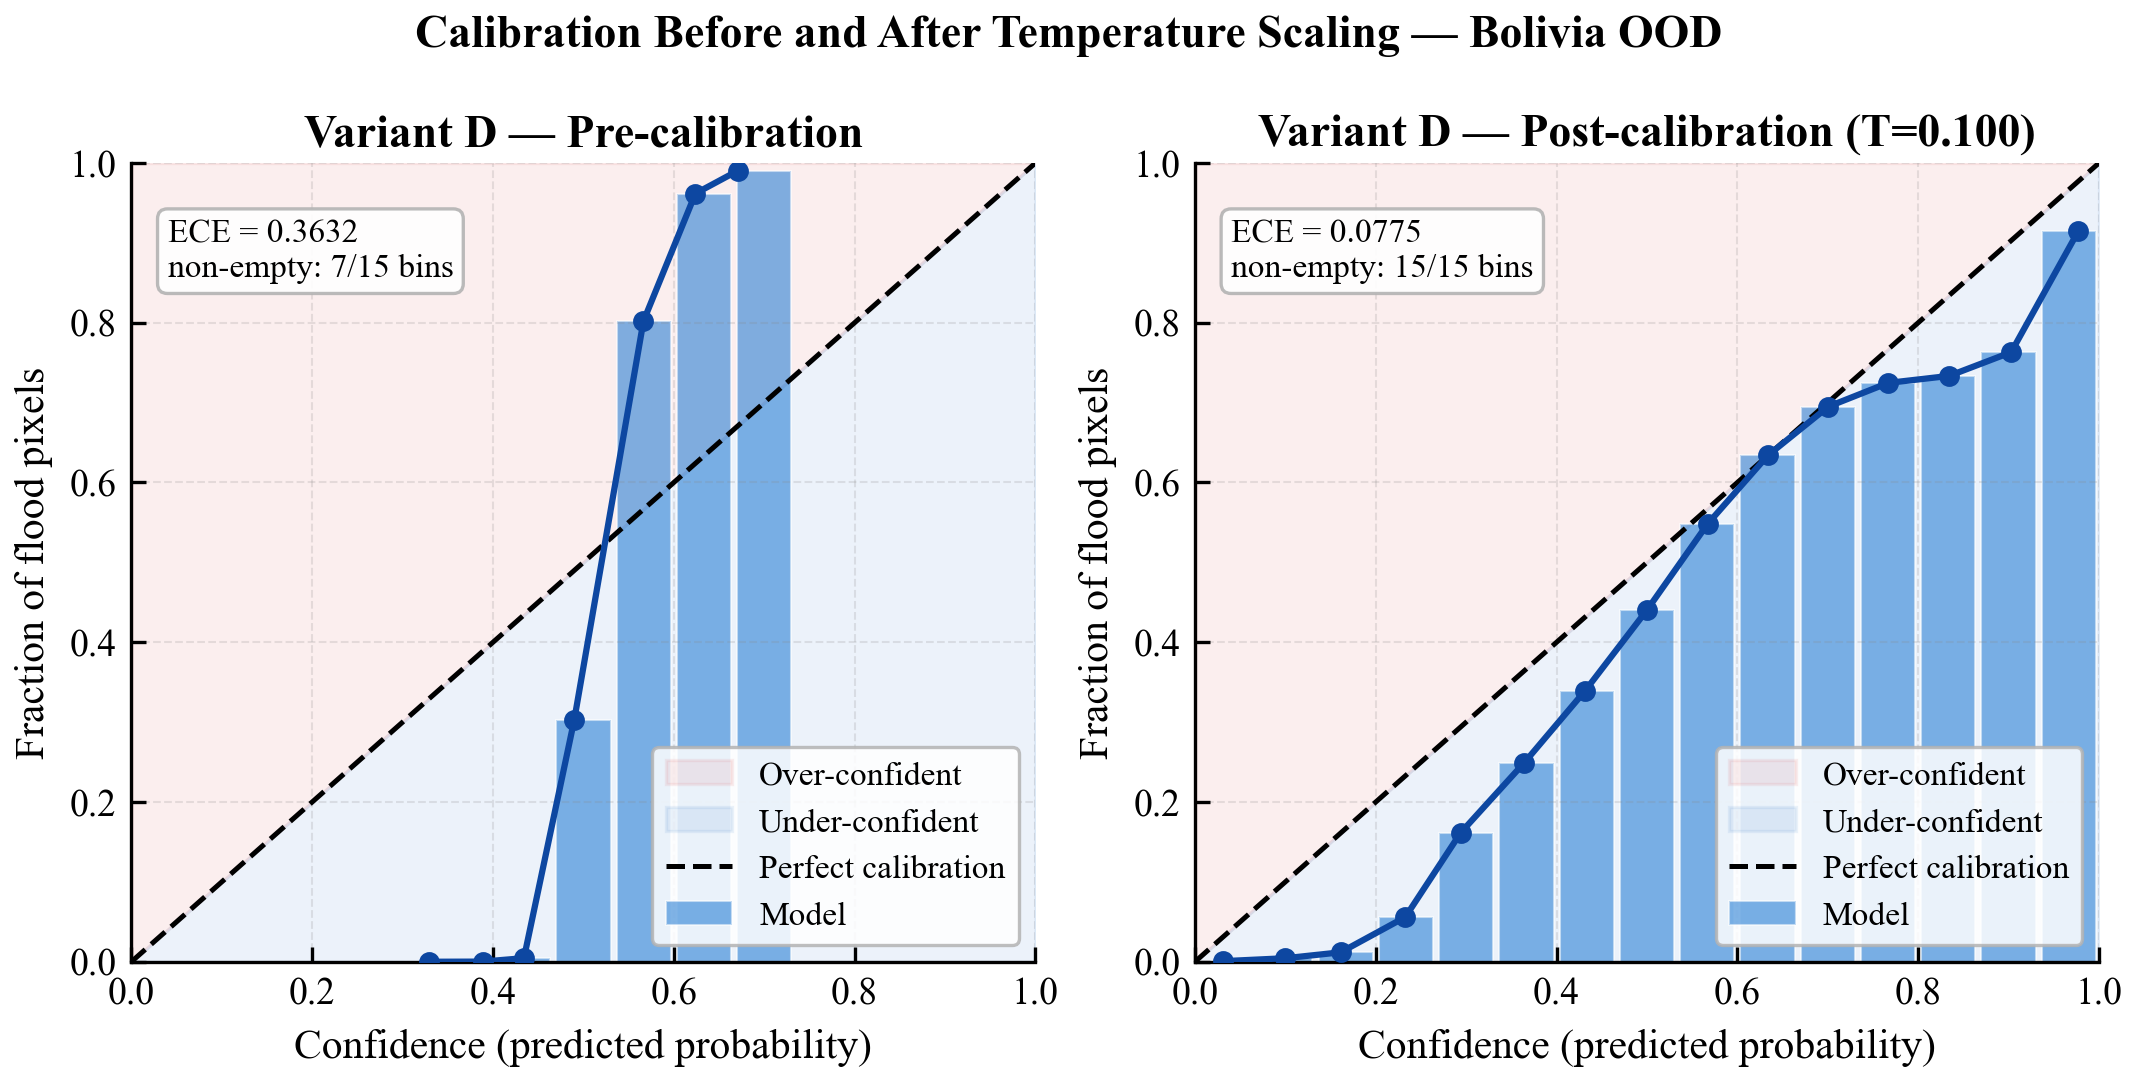
\includegraphics[width=0.88\textwidth]{fig_reliability_2panel}
\caption{Two-panel reliability diagram for Variant~D.  \textit{Left:}
pre-calibration reliability curve showing severe underconfidence
(predicted probabilities cluster near 0.5).  \textit{Right:} post-calibration
reliability curve ($T=0.100$) showing near-perfect alignment with the
diagonal.  Both panels include the weighted average ECE value and the
confidence histogram.}
\label{fig:reliability_2panel}
\end{figure}

\begin{figure}[h]
\centering
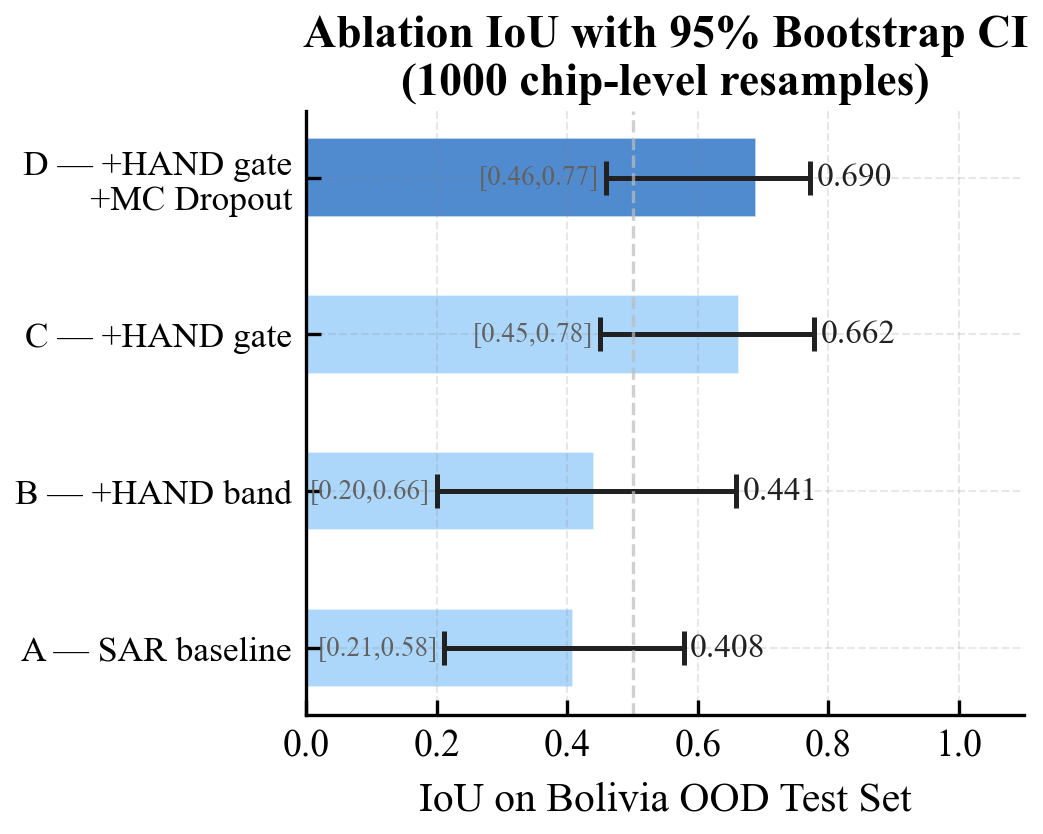
\includegraphics[width=0.85\textwidth]{fig_bootstrap_ci}
\caption{Bootstrap 95\% confidence intervals for the Bolivia test IoU
of Variants A, B, C, and D (1{,}000 chip-level resamples).  The overlapping
CIs for C and D illustrate the fundamental statistical challenge of evaluating
on only 15 test chips.}
\label{fig:bootstrap_ci}
\end{figure}

\begin{figure}[h]
\centering
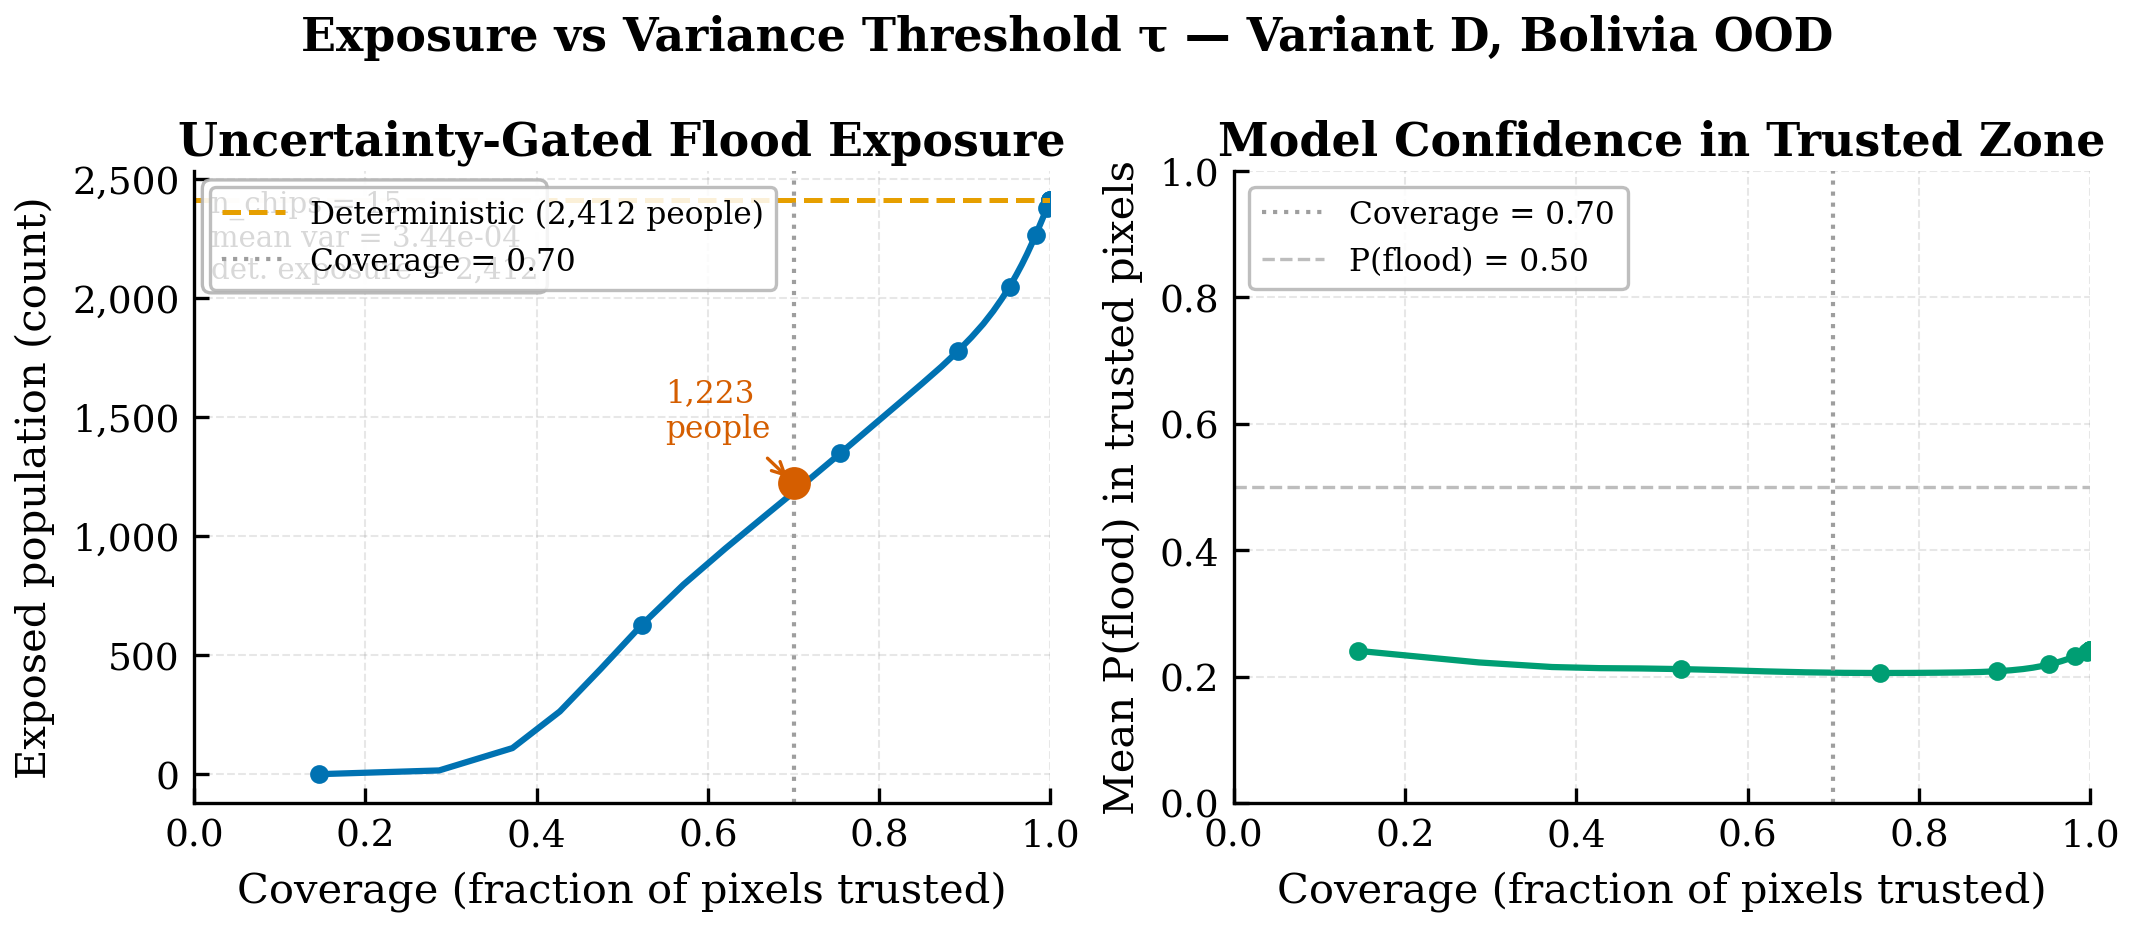
\includegraphics[width=0.75\textwidth]{fig_exposure_tau}
\caption{Sensitivity of the population exposure estimate to the uncertainty
threshold $\tau$.  With MC Dropout, the exposure is flat across all
$\tau \leq \hat{\sigma}^2_\text{max} \approx 0.001$—all pixels pass the
threshold regardless of $\tau$.  TTA uncertainty (pending) is expected to
produce a more responsive exposure–$\tau$ curve.}
\label{fig:exposure_tau}
\end{figure}

\begin{figure}[h]
\centering
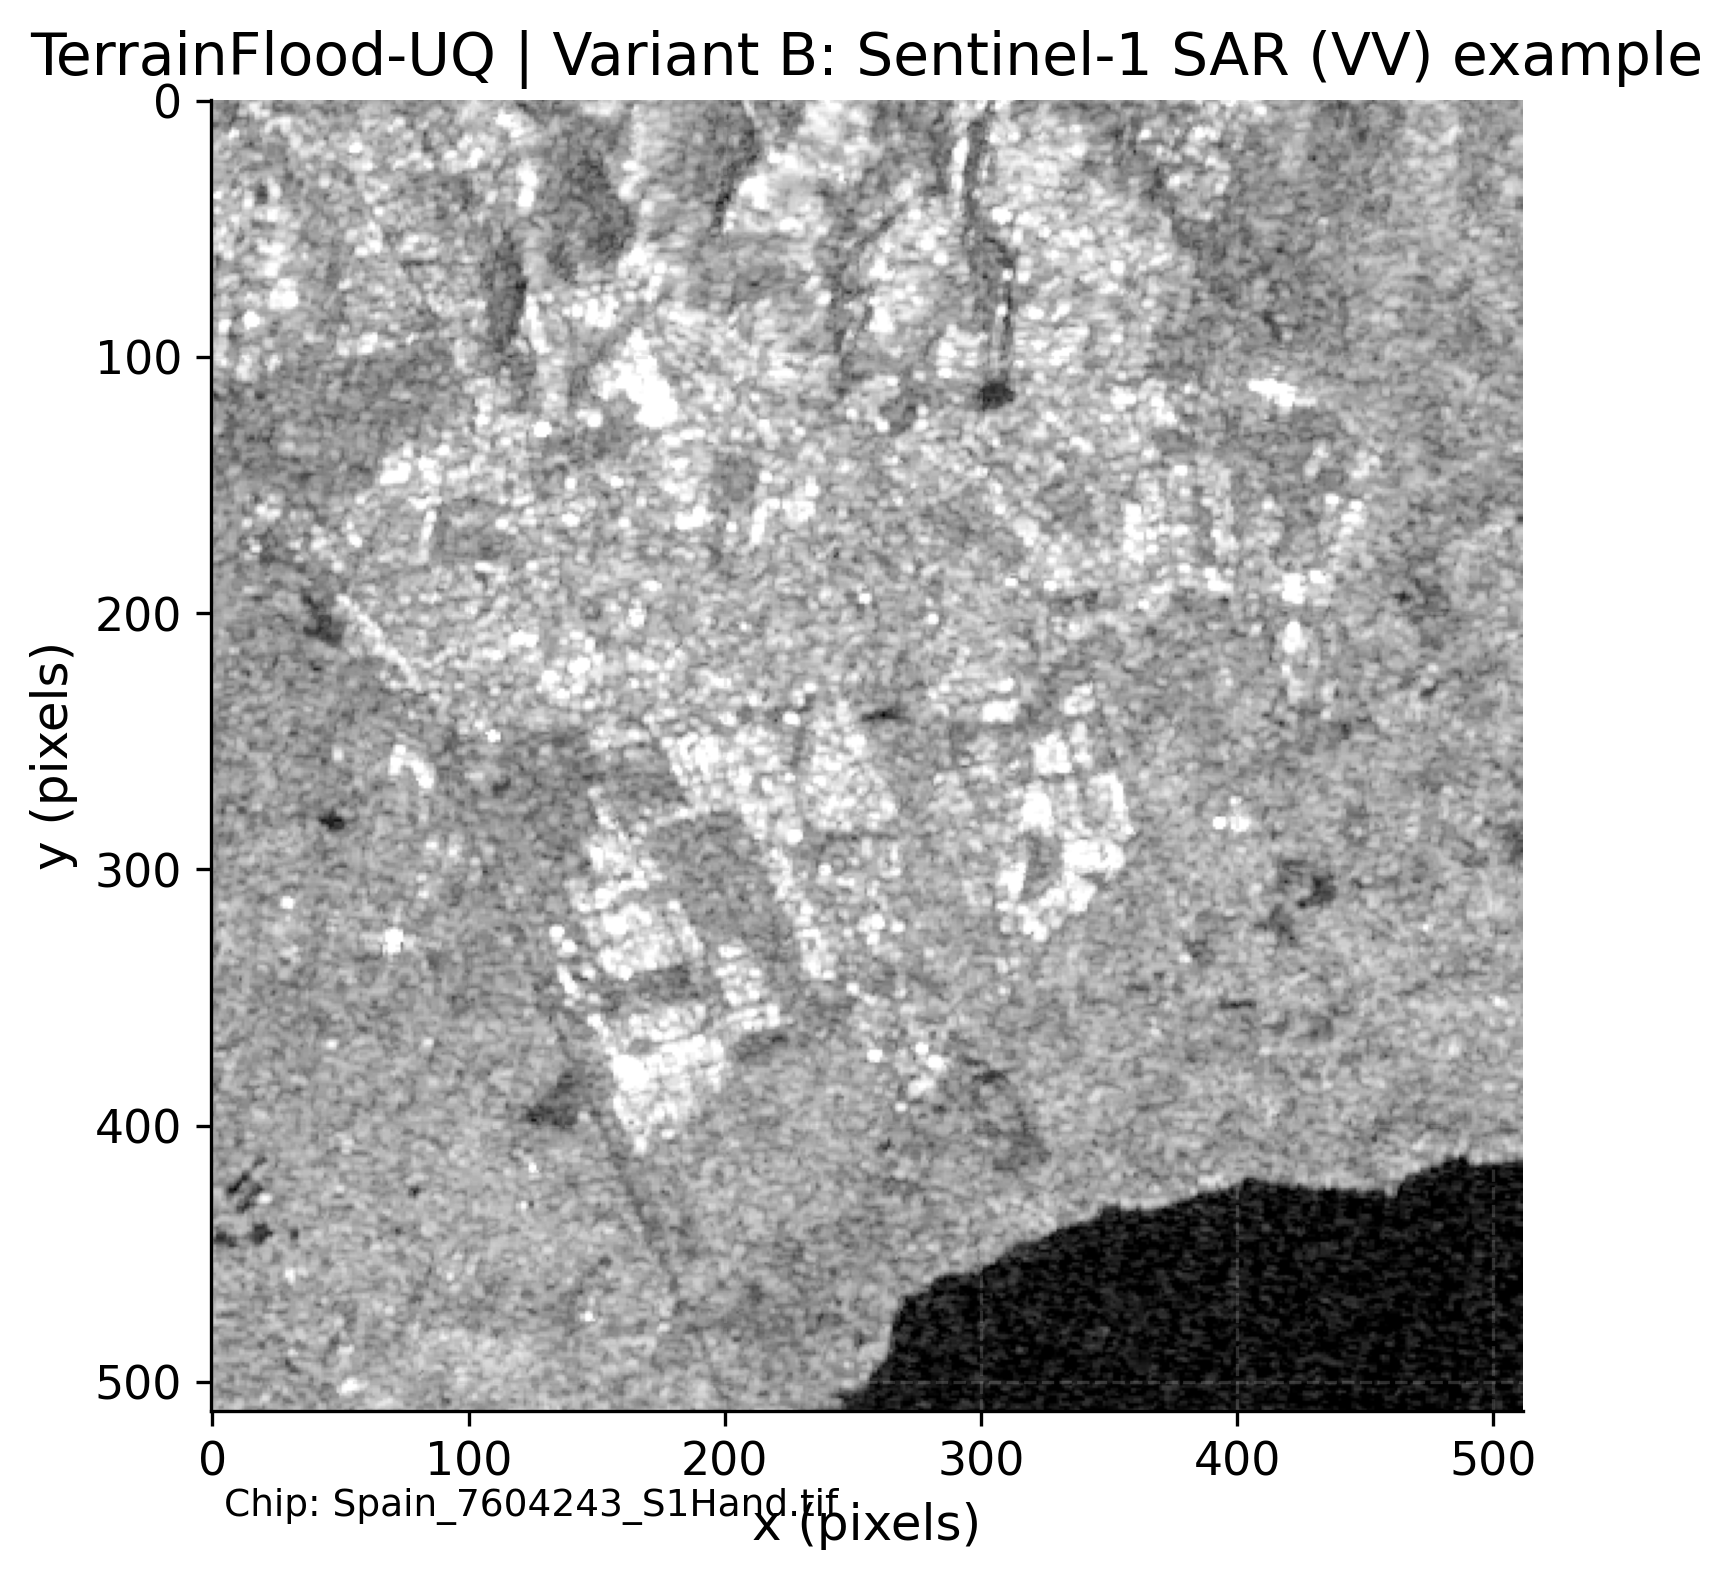
\includegraphics[width=0.90\textwidth]{fig1_sar_example}
\caption{Representative Sentinel-1 SAR imagery from the Bolivia flood
event.  \textit{Left:} VV post-event backscatter (dB)—open water appears
dark due to specular reflection.  \textit{Right:} VH post-event backscatter
(dB).  The contrast between flooded (dark) and dry (bright) pixels motivates
SAR-based flood detection.}
\label{fig:sar_example}
\end{figure}

\section{DKUCC Computing Environment}
\label{app:compute}

All model training and inference was conducted on the Duke Kunshan University
Computing Cluster (DKUCC) with NVIDIA L20 GPUs (48\,GB VRAM).  Jobs were
submitted via SLURM with the job scripts in \texttt{jobs/}.  The software
environment uses Anaconda 2023.7, CUDA 12.6, and PyTorch.
Table~\ref{tab:compute} summarises the compute budget.

\begin{table}[h]
\centering
\caption{Approximate compute budget per training job on DKUCC.}
\label{tab:compute}
\begin{tabular}{llr}
\toprule
\textbf{Job script} & \textbf{Description} & \textbf{Wall time} \\
\midrule
\texttt{train\_A.sbatch} & Variant A, 50 epochs  & $\leq$3\,h \\
\texttt{train\_B.sbatch} & Variant B, 50 epochs  & $\leq$4\,h \\
\texttt{train\_C.sbatch} & Variant C, 50 epochs  & $\leq$6\,h \\
\texttt{train\_D.sbatch} & Variant D, 50 epochs  & $\leq$8\,h \\
\texttt{train\_C\_full.sbatch} & Variant C, 120 ep., pat.25 & $\leq$12\,h \\
\texttt{train\_D\_full.sbatch} & Variant D, 120 ep., pat.25 & $\leq$14\,h \\
\texttt{run\_tta\_uncertainty.sbatch} & TTA + MC Dropout UQ  & $\leq$4\,h \\
\texttt{run\_eval\_all.sbatch} & Full evaluation pipeline & $\leq$6\,h \\
\bottomrule
\end{tabular}
\end{table}

\end{document}
